%\documentclass{pasj01}
\documentclass[proof]{pasj01}
%\draft
%%%%%%%%%%%%%%%%%%%%%%%%%%%%%%%%%%%%%%%%%%%%%%%%%%%%%%%%%%%%%%%%
%\usepackage[dvipdfmx]{graphicx}
\usepackage{listings}
\usepackage{color}
%\usepackage{amsmath}
\newcommand{\myvec}[1]{\vec{#1}}
\newcommand{\redtext}[1]{\textcolor{red}{#1}}
\newcommand{\icarus}{Icarus}
\newcommand{\pasa}{Publications of the Astronomical Society of Australia}
%%%%%%%%%%%%%%%%%%%%%%%%%%%%%%%%%%%%%%%%%%%%%%%%%%%%%%%%%%%%%%%%

\begin{document}

\title{Implementation and Performance of FDPS: A Framework for Developing
  Parallel Particle Simulation Codes}

\author{Masaki \textsc{Iwasawa}\altaffilmark{1}}
\email{masaki.iwasawa@riken.jp}
\altaffiltext{1}{RIKEN Advanced Institute for Computational Science,
7--1--26 Minatojima-minami-machi, Chuo-ku, Kobe, Hyogo, Japan}

\author{Ataru \textsc{Tanikawa}\altaffilmark{1,2}}
\email{tanikawa@ea.c.u-tokyo.ac.jp}
\altaffiltext{2}{Department of Earth and Astronomy, College of Arts and Science, The University of
Tokyo, 3--8--1 Komaba, Meguro-ku, Tokyo, Japan}
  
\author{Natsuki \textsc{Hosono}\altaffilmark{1}}
\email{natsuki.hosono@riken.jp}

\author{Keigo \textsc{Nitadori}\altaffilmark{1}}
\email{keigo@riken.jp}

\author{Takayuki \textsc{Muranushi}\altaffilmark{1}}
\email{takayuki.muranushi@riken.jp}

\author{Junichiro \textsc{Makino}\altaffilmark{3,1,4}}
\email{makino@mail.jmlab.jp}
\altaffiltext{3}{Department of Planetology, Graduate School of
  Science, Kobe University, 1-1, Rokkodai-cho, Nada-ku, Kobe, Hyogo,
  Japan}
\altaffiltext{4}{Earth-Life Science Institute, Tokyo Institute of
  Technology, 2--12--1 Ookayama, Meguro-ku, Tokyo, Japan}

\KeyWords{Methods: numerical --- Galaxy: evolution --- Cosmology: dark
  matter --- Planets and satellites: formation}

\maketitle

\begin{abstract}

We present the basic idea, implementation, measured performance and
performance model of FDPS (Framework for developing particle
simulators). FDPS is an application-development framework which helps
the researchers to develop simulation programs using particle methods
for large-scale distributed-memory parallel supercomputers. A
particle-based simulation program for distributed-memory parallel
computers needs to perform domain decomposition, exchange of particles
which are not in the domain of each computing node, and gathering of
the particle information in other nodes which are necessary for
interaction calculation. Also, even if distributed-memory parallel
computers are not used, in order to reduce the amount of computation,
algorithms such as Barnes-Hut tree algorithm or Fast Multipole Method
should be used in the case of long-range interactions. For short-range
interactions, some methods to limit the calculation to neighbor
particles are necessary. FDPS provides all of these functions which
are necessary for efficient parallel execution of particle-based
simulations as ``templates'', which are independent of the actual data
structure of particles and the functional form of the
particle-particle interaction. By using FDPS, researchers can write
their programs with the amount of work necessary to write a simple,
sequential and unoptimized program of $O(N^2)$ calculation cost, and
yet the program, once compiled with FDPS, will run efficiently on
large-scale parallel supercomputers. A simple gravitational $N$-body
program can be written in around 120 lines. We report the actual
performance of these programs and the performance model. The weak
scaling performance is very good, and almost linear speedup was
obtained for up to the full system of K computer. The minimum
calculation time per timestep is in the range of 30 ms ($N=10^7$) to
300 ms ($N=10^9$). These are currently limited by the time for the
calculation of the domain decomposition and communication necessary
for the interaction calculation. We discuss how we can overcome these
bottlenecks.

\end{abstract}

\section{Introduction}

Particle-based simulations have been widely used in the field of
computational science, and they are becoming more and more
popular. In particle-based simulations, a system under study is
regarded as a collection of mutually-interacting particles, or
a particle system,  and its
evolution is described by the evolution (in many cases, motion) of
individual particles. Examples of particle-based simulations include
gravitational $N$-body simulation, molecular dynamics simulation,
granular dynamics simulation, and element-free simulation of fluid
dynamics or structural analysis. In the case of molecular dynamics and
gravitational $N$-body simulations, the physical system under study is
a collection of particles, and the particle-based method is a natural
way to simulate the system. Element-free methods have advantages over
structured (or unstructured) grid-based method, depending on the
nature of the system and computer system to be used. 

In order to improve the resolution and accuracy of particle-based
simulations, it is necessary to utilize present-day HPC systems.
However, to develop a calculation code for particle systems
which can achieve high efficiency on present-day HPC systems is
difficult and time-consuming. There are several reasons for this
difficulty. In order to achieve high efficiency, we need to decompose
the computational domain, assign subdomains to computing nodes, and
redistribute particles according to their positions. This
decomposition should be dynamically changed to guarantee the good load
balance. This division of the computational domain means that
computing nodes need to exchange the information of particles to
evaluate the interactions on their particles. To achieve high
efficiency, the amount of the exchanged data must be minimized, and
interaction calculation should also be efficient, making good use of
cache memory and SIMD execution units. It is also important to make
use of GPGPUs or other types of accelerators, if available.

Domain decomposition and load balance have been discussed in a number
of works \cite{1994JCoPh.111..136S, 1996NewA....1..133D,
confscWarrenSBGSW97, 2004PASJ...56..521M, ishiyama:greem,
ishiyama:gordonbell}.  The efficient use of SIMD units is discussed
in \cite{2006NewA...12..169N,2012NewA...17...82T,2013NewA...19...74T},
and GPGPUs in \cite{hamada2009novel, 2009NewA...14..630G,
Hamada:2009:THN:1654059.1654123, Hamada:2010:TAN:1884643.1884644,
2012JCoPh.231.2825B, Bedorf:2014:PGT:2683593.2683600}.

Thus, to develop a code which has all of these necessary features for
present-day HPC systems has become a big project which requires
multi-year effort of a multi-person team. It has become difficult for
researchers outside such a team to try any new experiment which
requires nontrivial modification of the code. If one wants to develop
a new numerical scheme for particle-based simulation or to apply it to
new problem, it is necessary to write his/her own code. However, it is
practically impossible for a single person, or even for a group of
people, to develop a new code which can run efficiently on present-day
HPC systems in a reasonable time.  This difficulty, in our opinion, has
slowed down the evolution of the entire field of computational science
for the last two decades. Here we discussed the situation of
particle-based codes. The situation of grid-based codes is similar. 

In order to overcome the difficulty described above, we developed FDPS
(Framework for Developing Particle
Simulator)\footnote{https://github.com/FDPS/FDPS}. Our goal is to
provide a software framework which enables researchers and programmers
to develop high-performance particle simulation codes quickly. The
basic idea of FDPS is to separate the above-described ``difficult''
part of the code, such as the domain decomposition and exchange of
particles, from the description of the physical problem itself. The
difficult part is implemented in FDPS as a library. A user of FDPS
needs to define the data structure of particles and the interaction
function of particles. Then FDPS receives these code, and generates an
efficient code to perform domain decomposition and parallelized
calculation of interaction. The user program first uses the functions
of FDPS to do the interaction calculation, and then updates the
physical data of particles, and repeats this loop until the end of
simulation.  Thus, the user of FDPS does not have to write complex
code for parallelization.

FDPS supports particle simulations with arbitrary pairwise
interactions. If the physical system includes many-body interactions,
a user can calculate such interactions within his/her code, letting
FDPS do the parallelization and calculation of pairwise interactions.
In FDPS, the separation of parallelization and physical problem is
done through the use of abstract data types implemented using C++
templates. Users of FDPS provide actual particle data class and
interaction function to the class template defined in FDPS. Thus,
users can develop a gravitational $N$-body code, Smoothed Particle
Hydrodynamics (SPH) code, other particles-based fluid code,
large-scale molecular dynamics code, a Discrete Element Method (DEM)
code, and many other particle-based code using FDPS, and all of them
will automatically parallelized with near-optimal load balancing. A
similar approach to provide general-purpose framework is
in \cite{1995CoPhC..87..266W}, but it was limited to long-range
interaction with $1/r$ potential.

One might think that, even though it is not impossible to develop
general-purpose framework for parallel particle-based simulations,
such a framework would be inevitably  slow. Since the goal of FDPS is
to make efficient use of present-day HPC systems, we designed FDPS so
that it can achieve the performance not worse than that of existing
large-scale parallel codes for particle simulations. We will discuss
the achieved performance later.

The structure of this paper is as follows. In section~\ref{sec:user},
we overview how FDPS users implement a simulation code on FDPS.  In
section~\ref{sec:implementation}, we describe parallel algorithm
implemented in FDPS. In section~\ref{sec:performance}, we illustrate
how FDPS actually simplifies the development of user programs, using
two sample FDPS applications, and describe their performance. Finally,
we summarize this study in section~\ref{sec:conclusion}.

% LocalWords:  HPC subdomains SIMD GPGPUs multi FDPS parallelized SPH
% LocalWords:  parallelization


\section{How FDPS works}
\label{sec:user}

In this section, we describe the design concept of FDPS. In
section~\ref{sec:design}, we present the design concept of FDPS. In
section~\ref{sec:samplecode}, we show an $N$-body simulation code
written using FDPS, and describe how FDPS is used to perform
parallelization algorithms. Part of the contents in this scetion have been
published in \citet{2015FDPS}.

\subsection{Design and implementation}
\label{sec:design}

In this section, we describe the design and implementation of FDPS. We
first present the abstract view of calculation codes for particle-based
simulations on distributed-memory parallel computers, and then
describe how such abstraction is realized in FDPS.

\subsubsection{Abstract view of particle-based simulation codes}
\label{sec:view}

In a particle-based simulation code on a distributed-memory parallel
computer, which uses spatial decomposition to reduce communication,
time integration of the system proceeds in the following steps:
\begin{enumerate}
\item The entire computational domain is decomposed into subdomains,
  and usually one subdomain is assigned to one MPI
  process. Decomposition should achieve minimization of inter-node
  communication and good load-balance between nodes.
 \label{proc:decompose}

\item Particles are redistributed among the processes, so that each
  process owns particles in its subdomain.\label{proc:exchange}

\item Interactions between  particles are calculated.
   Each process  calculates interactions on its particles. To do so,
   it needs to receive the necessary data in other processes.
  \label{proc:interaction}

\item The data of particles are updated using the calculated
  interaction. This part is done without inter-process communication.
   \label{proc:local}
\end{enumerate}

Steps \ref{proc:decompose}, \ref{proc:exchange}, and
\ref{proc:interaction} involve parallelization and inter-process
communications. FDPS provides library functions to perform these parts. Therefore, 
users of FDPS do not have to write their own code to perform 
parallelization and inter-process communication.

Let us now explain how FDPS provides the libraries to perform steps
\ref{proc:decompose}, \ref{proc:exchange}, and
\ref{proc:interaction} for arbitrary systems of particles, in other
words, how FDPS provides the abstraction of these steps. 

The particle-based simulation codes for which FDPS can be used is
described by the initial value problem of the following set of 
ordinary differential equations:
\begin{align}
  \frac{d\myvec{u}_i}{dt} = \myvec{g}\left(\sum_j^N \myvec{f}
  (\myvec{u}_i, \myvec{u}_j), \myvec{u}_i\right), \label{eq:geq}
\end{align}
where $N$ is the number of particles in the system, $\myvec{u}_i$ is a
physical quantity vector of a particle, the function $\myvec{f}$
indicates the contribution of particle $j$ to the time derivative of
physical quantities of particle $i$, and $\myvec{g}$ is a function
which converts the sum of the contributions to actual time
derivative. For example, in the case of gravitational $N$-body
simulation, $\myvec{f}$ is the mutual gravity between particles,
$\myvec{g}$ would add, for example, the acceleration due to some
external field, and $\myvec{u}_j$ contains all necessary data of
particles such as position, velocity, mass, and other parameters.

Hereafter, we call a particle receiving the interaction
``$i$-particle'', and a particle exerting that interaction
``$j$-particle''. The actual content of vector $\myvec{u}_i$, and the
functional forms of $\myvec{f}$ and $\myvec{g}$ depends on the
physical system and how it is discretized.

Equation (\ref{eq:geq}) implies that FDPS can only handle pairwise
interactions which can be added to obtain the total contributions of
other particles. If many-body interaction is important, one can still
use FDPS to perform parallelization and calculation of pairwise
interactions. Many-body interaction, such as angle and torsion of
bonding force in molecular dynamics simulation, can be implemented in
the user code.

\subsubsection{Design concept of FDPS}
\label{sec:concept}

FDPS provides a template library in C++ language, which receives the
user-defined particle (vector $\myvec{u}_i$) and functions to
calculate pairwise interaction (function $\myvec{f}$). The functions
provided by this template library perform the steps
\ref{proc:decompose}, \ref{proc:exchange}, and \ref{proc:interaction}
described above. The function $\myvec{g}$, and the actual time
integration of $\myvec{u}_i$ are done entirely in the user
program. Thus, FDPS provides a powerful, and yet very flexible
framework for the development of calculation codes for particle-based
simulations.

\begin{figure}
  \begin{center}
    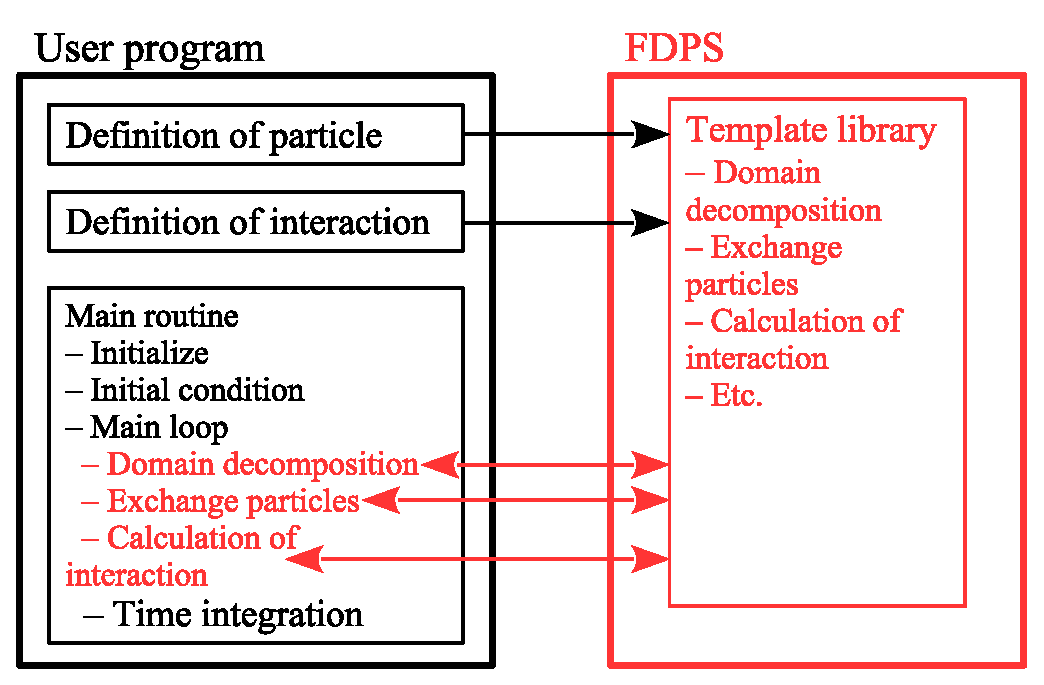
\includegraphics[width=8cm]{fig/concept.eps}
  \end{center}
  \caption{The basic concept of FDPS. The user program gives the
    definitions of particle and interaction to FDPS, and calls FDPS
    APIs.}
  \label{fig:concept}
\end{figure}

A user of FDPS can develop the simulation code in the following three
steps:
\begin{enumerate}
\item Define the data structure for $\myvec{u}_i$, as a class in C++
  language.
\item Define the function $\myvec{f}$. It should be a function object
  in C++ language\footnote{A function pointer of C language can be
    operable.}, which receives arrays of $i$-particles and
  $j$-particles, and calculates and accumulates $\myvec{f}$ on
  $i$-particles.
\item Write the user program using the data class and functions
  provided by FDPS. Currently, the user program should also be written
  in C++.
\end{enumerate}

Figure~\ref{fig:concept} illustrates how the user-defined code and
FDPS functions interact. The user program gives the definition of
particle and particle-particle interaction to FDPS at the compile
time. When executed, the user program first does the initialization
(the setup of MPI communication is done through a single call to an
FDPS initialization function), and the setup of the initial
condition. Then, the main integration loop is executed. In the main
loop, first the domain decomposition and exchange of particles are
performed, and then the calculation of interactions is
performed. These are all done through library calls to FDPS
functions. Finally, the time integration of particles using the
calculated interaction is performed.

In the above description, the interaction calculation is done once per
one iteration of the main loop. It is possible to use integration
schemes which requires multiple evaluations of interaction within a
single timestep, such as Runge-Kutta schemes. One can just call
interaction calculation API of FDPS, with $\myvec{u}_i$ containing
necessary intermediate values.

FDPS takes care of parallelization using MPI, and it can also use
OpenMP parallelization for internal operations and also for
interaction calculation. Thus, an FDPS user does not have to worry
about these issues. The efficient use of the cache memory and the SIMD
execution unit is not directly taken care by the FDPS libraries, but
handled through the interface to the user-defined interaction
calculation function. The interface is defined so that the interaction
calculation is done for multiple $j$-particles and multiple
$i$-particles. Thus, it performs a large amount of calculation, on a
small amount of data, since the calculation cost is the product of the
numbers of $i$- and $j$-particles, and data amount is sum of them.  In
order to make efficient use of the SIMD execution unit, the innermost
loop should be written in such a way that can be recognized as the
candidate of vectorization by the compiler used. The interface is
defined as taking AoS (array of structures) arguments.  Some compilers
for some architecture might not be able to generate the code to
utilize the SIMD unit for AoS data. In such a case, the user should
write the interaction function in which the AoS data is converted
internally to SoA (structure of arrays) data, and converted back to
the AoS form after the interaction is actually calculated.

\begin{figure}
  \begin{center}
    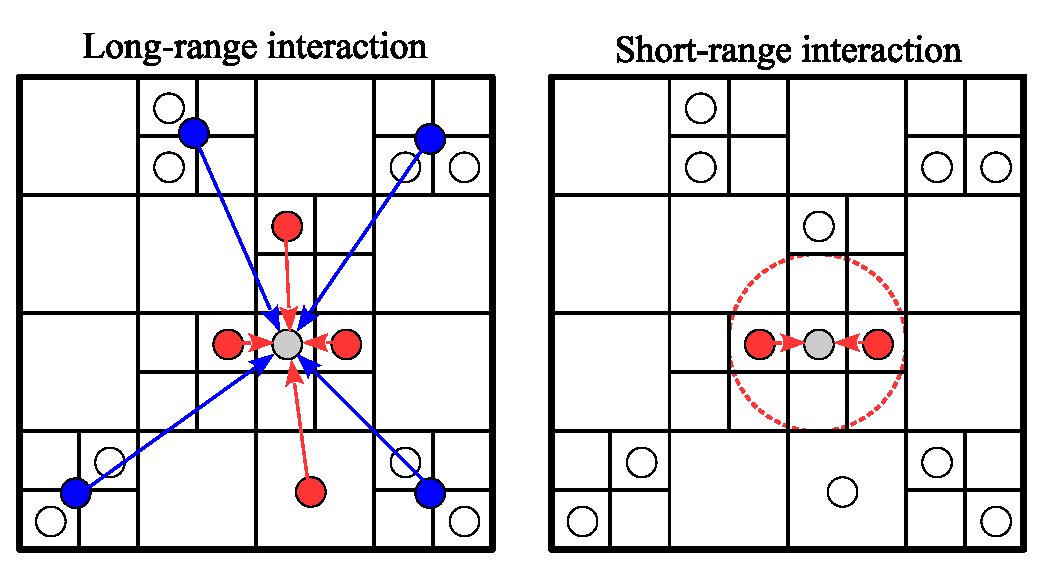
\includegraphics[width=8cm]{fig/force_type.eps}
  \end{center}
  \caption{Long-range interaction (left) and short-range interaction
    (right). Gray, red, and blue points are $i$-particle,
    $j$-particle, and superparticle, respectively.}
  \label{fig:forcetype}
\end{figure}

One might think that the definition of the system given in
equation~(\ref{eq:geq})  implies that  FDPS has to calculate $N^2$
interactions. If that were the case, FDPS would only be useful for
small problems. We implemented $O(N)$ and $O(N\log N)$ calculation
algorithms, for short-range and long-range interactions.

Within FDPS, the difference between long-range and short-range
interactions is slightly different from the physical one of infinite
and finite effective ranges. When we can and want to apply
multipole-like expansion to the contribution from distant particles,
we regard that interaction as long-range. The example of the
long-range interaction is gravity and Coulomb interaction in the open
boundary. When periodic boundary is used, they are usually evaluated
%using $\rm P^3M$ or PME method \cite{hockney1988computer}, in which
using $\mathrm{P^3M}$ or PME method \cite{hockney1988computer}, in
which the long-range part is evaluated using FFT, and only the
interaction with long-range cutoff is evaluated directly.  Even in
this case, we can still apply multipole interaction as used in TreePM
method \cite{1995ApJS...98..355X, 2000ApJS..128..561B,
  2002JApA...23..185B, 2004NewA....9..111D, springel:gadget2,
  2005PASJ...57..849Y, ishiyama:greem, ishiyama:gordonbell}, and in
this case the interaction is treated as long-range in FDPS.

For long-range interactions, FDPS uses standard Barnes-Hut tree
algorithm \cite{1986Natur.324..446B, 1990JCoPh..87..161B} parallelized
for distributed-memory machines and optimized for cache memory and
SIMD units \cite{ishiyama:greem, ishiyama:gordonbell}. For short-range
interactions, interaction list, or ``neighbor list'' for a group of
$i$ particles is constructed using a tree-based search, and that list
is used for the actual interaction calculation.
Figure~\ref{fig:forcetype} illustrates the long-range and short-range
interactions and how they are calculated in FDPS

For the long-range interaction, a multipole-like interaction is
used. Thus, equation~(\ref{eq:geq}) is modified to 
\begin{align}
  \frac{d\myvec{u}_i}{dt} = \myvec{g}\left( \sum_j^{N_{\mathrm{J},i}}
  \myvec{f}(\myvec{u}_i,\myvec{u}_j) + \sum_{j'}^{N_{\mathrm{S},i}}
  \myvec{f'}(\myvec{u}_i,\myvec{u'}_{j'}), \myvec{u}_i
  \right), \label{eq:geqL}
\end{align}
where $N_{\mathrm{J},i}$ and $N_{\mathrm{S},i}$ are, the number of
$j$-particles and superparticles for which we apply multipole-like
expansion, the vector $\myvec{u'}_{j'}$ is the physical quantity
vector of a superparticle, and the function $\myvec{f'}$ indicates the
interaction exerted on particle $i$ by the superparticle $j'$. In
simulations with a large number of particles $N$, $N_{\mathrm{J},i}$
and $N_{\mathrm{S},i}$ are many orders of magnitude smaller than $N$.
The user should also specify how superparticles are constructed from
ordinary particles, and also from superparticles in the lower level of
the tree. For $1/r$ potential, which is the typical usage of the
long-range interaction, FDPS provides the default way of construction
of superparticles up to the quadrupole moment.

In the case of the short-range interaction, the calculation of
contribution of distant particles is suppressed. Thus,
equation~(\ref{eq:geq}) is modified to
\begin{align}
  \frac{d\myvec{u}_i}{dt} = \myvec{g}\left(\sum_j^{N_{\mathrm{J},i}}
  \myvec{f}(\myvec{u}_i,\myvec{u}_j), \myvec{u}_i
  \right), \label{eq:geqS}
\end{align}
As in the case of the long-range force, $N_{\mathrm{J},i}$ is much
smaller than $N$, and usually independent of $N$.



% LocalWords:  FDPS subdomains subdomain MPI parallelization dt discretized API
% LocalWords:  APIs timestep Runge Kutta OpenMP SIMD vectorization AoS SoA PME
% LocalWords:  multipole FFT TreePM parallelized superparticles superparticle
% LocalWords:  quadrupole


\subsection{An example --- gravitational \textit{N}-body problem}
\label{sec:samplecode}

In this section, we present the complete working example of a
simulation code written using FDPS, to illustrate how a user actually
uses FDPS. As the target problem, we use the gravitational $N$-body
problem with an open boundary.  Within the terminology of FDPS, the
interaction between particles in the gravitational $N$-body problem is
of the ``long-range'' type. Therefore, we need to specify the function
to calculate interactions for both the ordinary particles and
superparticles. For the sake of brevity, we use the center-of-mass
approximation for superparticles, which means we can actually use the
same function for both types of particles.

The physical quantity vector $\myvec{u}_i$ and interaction functions
$\myvec{f}$, $\myvec{f'}$, and $\myvec{g}$ for the gravitational
$N$-body problem is now given by:
\begin{align}
  \myvec{u}_i &= (\myvec{r}_i,
  \myvec{v}_i,m_i) \label{eq:PhysicalVectorNbody} \\
%%  
  \myvec{f} (\myvec{u}_i, \myvec{u}_j) &= \frac{Gm_j \left(
    \myvec{r}_j - \myvec{r}_i \right)}{ \left( |\myvec{r}_j -
    \myvec{r}_i|^2 + \epsilon_i^2
    \right)^{3/2}} \label{eq:ParticleParticleNbody} \\
%%
  \myvec{f'} (\myvec{u}_i, \myvec{u'}_j) &= \frac{Gm_j' \left(
    \myvec{r}_j - \myvec{r'}_i \right)}{ \left( |\myvec{r}_j -
    \myvec{r'}_i|^2 + \epsilon_i^2
    \right)^{3/2}} \label{eq:ParticleSuperparticleNbody} \\
%%
  \myvec{g}(\myvec{F},\myvec{u}_i)  &= (\myvec{v}_i,\myvec{F},0),
\label{eq:ConversionNbody}
\end{align}
where $m_i$, $\myvec{r}_i$, $\myvec{v}_i$, and $\epsilon_i$ are, the
mass, position, velocity, and gravitational softening of particle $i$,
$m_j'$ and $\myvec{r'}_j$ are, the mass and position of a
superparticle $j$, and $G$ is the gravitational constant.  Note that
the shapes of the functions $\myvec{f}$ and $\myvec{f'}$ are the same.

Listing~\ref{code:samplecode} shows the complete code which can be
actually compiled and run, not only on a single-core machine but also
massively-parallel, distributed-memory machines such as the full-node
configuration of the K computer. The total number of lines is only
117.


\begin{lstlisting}[label=code:samplecode,numbers=left,numbersep=5pt,frame=single,basicstyle=\ttfamily,caption=A sample code of $N$-body simulation]
#include <particle_simulator.hpp>
using namespace PS;

class Nbody{
public:
    F64    mass, eps;
    F64vec pos, vel, acc;
    F64vec getPos() const {return pos;}
    F64 getCharge() const {return mass;}
    void copyFromFP(const Nbody &in){ 
        mass = in.mass;
        pos  = in.pos;
        eps  = in.eps;
    }
    void copyFromForce(const Nbody &out) {
        acc = out.acc;
    }    
    void clear() {
        acc = 0.0;
    }
    void readAscii(FILE *fp) {
        fscanf(fp,
               "%lf%lf%lf%lf%lf%lf%lf%lf",
               &mass, &eps,
               &pos.x, &pos.y, &pos.z,
               &vel.x, &vel.y, &vel.z);
    }
    void predict(F64 dt) {
        vel += (0.5 * dt) * acc;
        pos += dt * vel;
    }
    void correct(F64 dt) {
        vel += (0.5 * dt) * acc;
    }
};

template <class TPJ>
struct CalcGrav{
    void operator () (const Nbody * ip,
                      const S32 ni,
                      const TPJ * jp,
                      const S32 nj,
                      Nbody * force) {
        for(S32 i=0; i<ni; i++){
            F64vec xi  = ip[i].pos;
            F64    ep2 = ip[i].eps
                * ip[i].eps;
            F64vec ai = 0.0;
            for(S32 j=0; j<nj;j++){
                F64vec xj = jp[j].pos;
                F64vec dr = xi - xj;
                F64 mj  = jp[j].mass;
                F64 dr2 = dr * dr + ep2;
                F64 dri = 1.0 / sqrt(dr2);                
                ai -= (dri * dri * dri
                       * mj) * dr;
            }
            force[i].acc += ai;
        }
    }
};

template<class Tpsys>
void predict(Tpsys &p,
             const F64 dt) {
    S32 n = p.getNumberOfParticleLocal();
    for(S32 i = 0; i < n; i++)
        p[i].predict(dt);
}

template<class Tpsys>
void correct(Tpsys &p,
             const F64 dt) {
    S32 n = p.getNumberOfParticleLocal();
    for(S32 i = 0; i < n; i++)
        p[i].correct(dt);
}

template <class TDI, class TPS, class TTFF>
void calcGravAllAndWriteBack(TDI &dinfo,
                             TPS &ptcl,
                             TTFF &tree) {
    dinfo.decomposeDomainAll(ptcl);
    ptcl.exchangeParticle(dinfo);    
    tree.calcForceAllAndWriteBack
        (CalcGrav<Nbody>(),
         CalcGrav<SPJMonopole>(),
         ptcl, dinfo);    
}

int main(int argc, char *argv[]) {
    F32 time  = 0.0;
    const F32 tend  = 10.0;
    const F32 dtime = 1.0 / 128.0;
    PS::Initialize(argc, argv);
    PS::DomainInfo dinfo;
    dinfo.initialize();
    PS::ParticleSystem<Nbody> ptcl;
    ptcl.initialize();
    PS::TreeForForceLong<Nbody, Nbody,
        Nbody>::Monopole grav;
    grav.initialize(0);
    ptcl.readParticleAscii(argv[1]);
    calcGravAllAndWriteBack(dinfo,
                            ptcl,
                            grav);
    while(time < tend) {
        predict(ptcl, dtime);        
        calcGravAllAndWriteBack(dinfo,
                                ptcl,
                                grav);
        correct(ptcl, dtime);        
        time += dtime;
    }
    PS::Finalize();
    return 0;
}
\end{lstlisting}


Now let us explain how this sample code works. This code consists of
four parts: The declaration to use FDPS (lines 1 and 2), the
definition of the particle (the vector $\myvec{u}_i$) (lines 4 to 35),
the definition of the gravitational force (the functions $\myvec{f}$
and $\myvec{f'}$) (lines 37 to 61), and the actual user program,
comprising a user-defined main routine and user-defined functions from
which library functions of FDPS are called (lines 63 to line 117). In
the following, we explain them step by step.

In order to declare to use FDPS, the only thing the user program need
to do is to include the header file ``particle\_simulator.hpp''. This
file and other source library files of FDPS should be in the include
path of the compiler. Everything in the standard FDPS library is
provided as the header source library, since they are implemented as
template libraries which need to receive particle class and
interaction functions. Everything in FDPS is provided in the namespace
``PS''. Therefore in this sample program, we declare it as the default
namespace to simplify the code. (For simplicity's sake, we do not omit
the namespace ``PS'' of FDPS functions and class templates in the main
routine.)

Before going to the 2nd parts, let us list the data types and classes
defined in FDPS. \texttt{F32/F64} are data types of 32-bit and 64-bit
floating points. \texttt{S32} is a data type of 32-bit signed integer.
\texttt{F64vec} is a class of a vector consisting of three 64-bit
floating points. This class provides several operators, such as the
addition, subtraction and the inner product indicated by ``$*$''.
Users need not use these data types in their own program, but some of
the functions which users should define should return the values in
these data types.

In the 2nd part, we define the particle, i.e. the vector
$\myvec{u}_i$, as a class \texttt{Nbody}. This class has member
variables: \texttt{mass} ($m_i$), \texttt{eps}
($\epsilon_i$), \texttt{pos} ($\myvec{r}_i$), \texttt{vel}
($\myvec{v}_i$), and \texttt{acc} ($d\myvec{v}_i/dt$). Although the
member variable \texttt{acc} does not appear in
equation~(\ref{eq:PhysicalVectorNbody}) -- (\ref{eq:ConversionNbody}),
we need this variable to store the result of the gravitational force
calculation. A particle class for FDPS must provide public member
functions \texttt{getPos}, \texttt{getCharge}, \texttt{copyFromFP},
\texttt{copyFromForce}, \texttt{clear},
and \texttt{readAscii}, in these names, so that the internal functions
of FDPS can access the data within the particle class.  For the name
of the particle class itself and the names of the member variables, a
user can use whatever names allowed by the C++ syntax.  The member
functions \texttt{predict} and \texttt{correct} are used in the
user-defined part of the code to integrate the orbits of particles.
Note that since the interaction used here is of $1/r$ type, the
definition and construction method of the superparticle are given as
the default in FDPS and not shown here.

In the 3rd part, the interaction functions $\myvec{f}$ and
$\myvec{f'}$ are defined. Since the shapes of the functions
$\myvec{f}$ and $\myvec{f'}$ are the same, we give one as a template
function.  The interaction function used in FDPS should have the
following five arguments. The first argument \texttt{ip} is the
pointer to the array of variables of particle
class \texttt{Nbody}. This argument specifies $i$-particles which
receive the interaction. The second argument \texttt{ni} is the number
of $i$-particles. The third argument \texttt{jp} is the pointer to the
array of variable of a template data type \texttt{TPJ}. This argument
specifies $j$-particles or superparticles which exert the
interaction. The fourth argument \texttt{nj} is the number of
$j$-particles or super-particles. The fifth argument \texttt{force} is
the pointer to the array of a variable of a user-defined class to
which the calculated interaction on an $i$-particle can be stored. In
this example, we used the particle class itself, but this can be
another class or a simple array.

%
The interaction function should be defined as a function object, so
that it can be passed to other functions as argument. Thus, it is
declared as a \texttt{struct}, with the only member
function \texttt{operator ()}.  In this example, the interaction is
calculated through a simple double loop. In order to make full
advantage of the SIMD unit in modern processors,
architecture-dependent tuning may be necessary, but only to this
single function.

In the 4th part, we give the main routine and functions called from
the main routine. In the following, we describe the main routine in
detail, and briefly discuss other functions. The main routine consists
of the following seven steps:
\begin{enumerate}
\item Set simulation time and timestep (lines 92 to 94). \label{proc:literal}
\item Initialize FDPS (line 95). \label{proc:init}
\item Create and initialize objects of FDPS classes (lines 96 to 102). \label{proc:construct}
\item Read in particle data from a file (line 103). \label{proc:input}
\item Calculate the gravitational forces of all the particles at the
  initial time (lines 104 to 106). \label{proc:calcinteraction}
\item Integrate the orbits of all the particles with Leap-Frog method
  (lines 107 to 114). \label{proc:integration}
\item Finish the use of  FDPS (line 115). \label{proc:fin}
\end{enumerate}

In the following, we describe  steps~\ref{proc:init},
\ref{proc:construct}, \ref{proc:input}, \ref{proc:calcinteraction},
and \ref{proc:fin}, and skip steps~\ref{proc:literal}
and \ref{proc:integration}.  In step~\ref{proc:literal}, we do not
call FDPS libraries.  Although we call FDPS libraries in
step~\ref{proc:integration}, the usage is the same as in
step~\ref{proc:calcinteraction}.

In step~\ref{proc:init}, the FDPS function \texttt{Initialize} is
called. In this function, MPI and OpenMP libraries are initialized. If
neither of them are used, this function does nothing.  All functions
of FDPS must be called between this function and the
function \texttt{Finalize}.

In step~\ref{proc:construct}, we create and initialize three objects
of the FDPS classes:
\begin{itemize}
\item \texttt{dinfo}: An object of class \texttt{DomainInfo}. It is
  used for domain decomposition.
\item \texttt{ptcl}: An object of class template \texttt{ParticleSystem}.
It takes the user-defined particle class (in this
example, \texttt{Nbody}) as the template argument. From the user
program, this object looks as an array of $i$-particles.
\item \texttt{grav}: An object of a data type \texttt{Monopole} defined in
a class template \texttt{TreeForForceLong}. This object is used for
the calculation of long-range interaction using the tree algorithm.
It receives three user-defined classes template arguments: the class
to store the calculated interaction, the class for $i$-particles and
the class for $j$-particles. In this example, all three are the same
as the original class of particles.  It is possible to define classes
with minimal data for these purposes and use them here, in order to
optimize the cache usage. The data type \texttt{Monopole} indicates
that the center-of-mass approximation is used for superparticles.
\end{itemize}

In step~\ref{proc:input}, the data of particles are read from a file
into the object \texttt{ptcl}, using the FDPS
function \texttt{readParticleAscii}. In the function, a member
function of class \texttt{Nbody}, \texttt{readAscii}, is called.

In step~\ref{proc:calcinteraction}, the forces on all particles are
calculated through the function \texttt{calcGravAllAndWriteBack}, which
is defined in lines 79 to 89. In this function,
steps~\ref{proc:decompose}, \ref{proc:exchange}, and
\ref{proc:interaction} in section~\ref{sec:view} are performed. In
other words, all of the actual work of FDPS libraries to calculate
interaction between particles takes place here. For
step~\ref{proc:decompose}, \texttt{decomposeDomainAll}, a member function
of class \texttt{DomainInfo} is called. This function takes the object
\texttt{ptcl} as an argument to use the positions of particles to
determine the domain decomposition.  Step~\ref{proc:exchange} was
performed in \texttt{exchangeParticle}, a member function of
class \texttt{ParticleSystem}. This function takes the
object \texttt{dinfo} as an argument and redistributes particles among
MPI processes.  Step~\ref{proc:interaction} was performed
in \texttt{calcForceAllAndWriteBack}, a member function of
class \texttt{TreeForForceLong}. This function takes the user-defined
function object \texttt{CalcGrav} as the first and second arguments,
and calculates particle-particle and particle-superparticle
interactions using them.

In step~\ref{proc:fin}, the FDPS function \texttt{Finalize} is
called. It calls the \texttt{MPI\_finalize} function.

In this section, we have described in detail how a user program
written using FDPS looks like. As we stated earlier, this program can
be compiled with or without parallelization using MPI and/or OpenMP,
without any change in the user program. The executable parallelized
with MPI is generated by using an appropriate compiler with MPI
support and a compile-time flag.  Thus, a user need not worry about
complicated bookkeeping necessary for parallelization using MPI.
%
In the next section, we describe how FDPS provides a generic
framework which takes care of parallelization
and bookkeeping for particle-based simulations. 

% LocalWords:  monopole superparticle FDPS hpp namespace nd th vec Nbody eps dt
% LocalWords:  pos vel acc getPos getCharge copyFromFP copyFromForce readAscii
% LocalWords:  ip const ni jp TPJ nj MPI OpenMP DomainInfo dinfo subdomains
% LocalWords:  subdomain ParticleSystem ptcl TreeForForceLong readParticleAscii
% LocalWords:  calcGravAllAndWriteBack decomposeDomainAll exchangeParticle SIMD
% LocalWords:  calcForceAllAndWriteBack CalcGrav superparticles struct grav
% LocalWords:  parallelization parallelized timestep


\section{Implementation}
\label{sec:implementation}

In this section, we describe how the operations discussed in the
previous section are implemented in FDPS. In
section~\ref{sec:decomposition} we describe the domain decomposition
and particle exchange, and in section~\ref{sec:calculation}, the
calculation of interactions. Part of the contents in this scetion have
been published in \citet{2015FDPS}.

\subsection{Domain decomposition and particle exchange}
\label{sec:decomposition}

In this section, we describe how the domain decomposition and the
exchange of particles are implemented in FDPS. We used the
multisection method
\citep{2004PASJ...56..521M} with the so-called sampling
method \citep{Blackston:1997:HPE:509593.509597}. The multisection
method is a generalization of ORB (Orthogonal Recursive Bisection). In
ORB, as its name suggests, bisection is applied to each coordinate
axis recursively. In multisection method, division in one coordinate
is not to two domains but to an arbitrary number of domains. Since one
dimension can be divided to more than two sections, it is not
necessary to apply divisions many times. So we apply divisions only
once to each coordinate axis. A practical advantage of this method is
that the number of processors is not limited to powers of two.

Figure~\ref{fig:decomposition} illustrates an example of the
multisection method with $(n_x, n_y, n_z)=(7,6,1)$. We can see that
the size and shape of subdomains show large variation. By allowing
this variation, FDPS achieves quite good load balance and high
scalability. Note that $n=n_x n_y n_z$ is the number of MPI
processes. By default, values of $n_x$, $n_y$, and $n_z$ are chosen so
that they are integers close to $n^{1/3}$. For figure
~\ref{fig:decomposition}, we force the numbers used to make a
two-dimensional decomposition.

\begin{figure}
  \begin{center}
    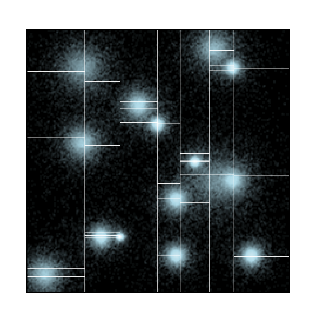
\includegraphics[width=8cm]{figure/pm3d.eps}
  \end{center}
  \caption{Example of the domain decomposition. The division is $7
    \times 6$ in 2-dimension.}
  \label{fig:decomposition}
\end{figure}


In the sampling method, first each process performs random sampling of
particles under it, and sends them to the process with rank 0
(``root'' process hereafter). Then the root process calculates the
division so that sample particles are equally divided over all
processes, and broadcasts the geometry of domains to all other
processes. In order to achieve good load balance, sampling frequency
should be changed according to the calculation cost per particle
\citep{2009PASJ...61.1319I}.

The sampling method works fine, if the number of particles per process
is significantly larger than the number of process. This is, however,
not the case for runs with a large number of nodes.  When the number
of particles per process is not much larger than the number of
processes, the total number of sample particles which the root process
needs to handle exceeds the number of particles per process itself,
and thus calculation time of domain decomposition in the root process
becomes visible.

%For example, K computer has more than 80,000 nodes, and in this paper
%we report the result of runs with all nodes. Even with Even with the
%number of particles per process same as the number of nodes, the
%total number of particles becomes 6.4 billion, and we do want to run
%simulations with smaller number of particles.

In order to reduce the calculation time, we also parallelized the
domain decomposition, currently in the direction of $x$ axis only. The
basic idea is that each node sends the sample particles not to the
root process of the all MPI processes but to the processes with index
$(i,0,0)$. Then processes $(i,0,0)$ sort the sample particles and
exchange the number of sample particles they received. Using these two
pieces of information, each of $(i,0,0)$ processes can determine all
domain boundaries inside its current domain in the $x$ direction. Thus,
they can determine which sample particles should be sent to
where. After the exchange of sample particles, each of $(i,0,0)$
processes can determine the decompositions in $y$ and $z$ directions.

A naive implementation of the above algorithm requires ``global''
sorting of sample particles over all of $(i,0,0)$ processes. In order
to simplify this part, before each process sends the sample particles
to  $(i,0,0)$ processes, they exchange their samples with other
processes with the same location in $y$ and $z$ process coordinates, so
that they have sample particles in the current domain decomposition in
the x direction. As a result, particles sent to $(i,0,0)$ processes
are already sorted at the level of domains decomposition in $x$
direction, and we need only the  sorting within each of $(i,0,0)$
processes to obtain the globally sorted particles.

Thus, our implementation of parallelized domain decomposition
is as follows:

\begin{enumerate}
\item
Each process samples particles randomly from its own particles. In
order to achieve an optimal load balance, the sampling rate of
particles is changed so that it is proportional to the CPU time per
particle spent on that process \citep{2009PASJ...61.1319I}. FDPS
provides several options including this optimal
balance. \label{prcoc:sampling}

%%
\item
Each process exchanges the sample particles according to the current
domain boundary in the $x$ direction with the process with the same y
and z indices, so that they have sample particles in the current
domain decomposition in the $x$ direction.


\label{proc:commx}

%%
\item
Each process with index $(i,y,z)$ sends the sample particles to the
process with index $(i,0,0)$, in other words, the root processes in
each of $y$-$z$ planes collects subsamples.

\label{proc:gatherx}

%%
\item
Each root process sorts the sample particles in the $x$ direction. Now,
the sample particles are sorted globally in the $x$ direction.

%%
\item
Each root process sends the number of the sample particles to the
other root processes and determines the global rank of the sample
particles.

%%
\item
Determine the $x$ coordinate of new domains by dividing all sample
particles into $n_x$ subsets with equal number of sample particles.
\label{proc:determinex}

%%
\item
Each root process exchanges sample particles with other root
processes, so that they have the sample particles in new domain in the
$x$ direction.

%\ref{proc:determinex}.

%of which $x$ coordinate is in the range of
%the $x$ coordinate of new subdomain determined in
%step

%%
\item
Each root process determines the $y$ and $z$ coordinates of new domains.
\label{proc:detyz}

%%
\item
Each root process broadcasts the geometries of new domains to all
other processes.
\label{proc:broadcasting}

\end{enumerate}

It is also possible to parallelize  the determination of  subdomains in
step \ref{proc:detyz}, but even for the full-node runs on K computer
we found the current parallelization is sufficient.

For particle exchange and also for interaction information exchange,
we use {\tt MPI\_Alltoall} to exchange the length of the data and {\tt
MPI\_Isend} and {\tt MPI\_Irecv} to actually exchange the data. At
least on K computer, we found that the performance of vendor-provided
{\tt MPI\_Alltoall} is not optimal for short messages. We implemented
a hand-crafted version in which the messages sent to the same relay
points are combined in order to reduce the total number of messages.


After the domain decomposition is done and the result is broadcasted
to all processes, they exchange particles so that each of them has
particles in its domain. Since each process has the complete
information of the domain decomposition, this part is pretty
straightforward to implement. Each process looks at each of its
particles, and determines if that particle is still in its domain.  If
not, the process determines to which process that particle should be
sent. After the destinations of all particles are determined, each
process sends them out, using {\tt MPI\_Isend} and {\tt MPI\_Irecv}
functions.


% LocalWords:  FDPS subdomain MPI multi subdomains DomainInfo ParticleSystem
% LocalWords:  decomposeDomainAll exchangeParticle substeps scalability
% LocalWords:  broadcasted Alltoallv


\subsection{Interaction calculation}
\label{sec:calculation}

In this section, we describe the implementation of the calculation of
interactions in FDPS. Conceptually, it consists of the following two
steps. In the first step, each process determines, for each of other
processes, which of its particles and superparticles are required by
that process for interaction calculation, and sends them to it. In the
second step, each process calculates the interactions onto
$i$-particles by calling user-defined function objects.

\if 0
\begin{enumerate}
\item Each process determines, for each of other processes, which of
  its particles and   superparticles are required by that process for
  interaction calculation,   and sends them to it.

%%
\item Each process calculates the interactions onto  $i$-particles by
  calling user-defined function objects.
\end{enumerate}
\fi

\begin{figure}
  \begin{center}
    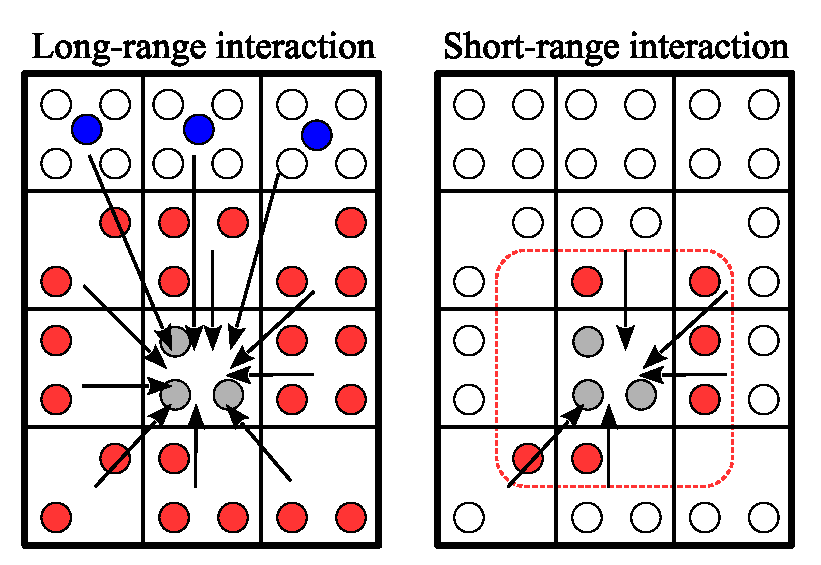
\includegraphics[width=8cm]{fig/exchangeLET.eps}
  \end{center}
  \caption{Illustration of communication among processes during the
    interaction calculation.}
  \label{fig:exchangeLET}
\end{figure}

For both steps, the octree structure is used, both for long- and
short-range interactions.
%%In step 1, 
In the first step, each process constructs the tree structure for its
local particles, and uses it to determine what data should be sent to
other processes. For the long-range interactions, this part is done
through the usual tree traversal \cite{1986Natur.324..446B,
  1990JCoPh..87..161B}. For the short-range interactions, tree
traversal is also used. A cube in a tree need to be subdivided if it
is within the cutoff length from anywhere in the domain of the process
to which the data will be sent.  The current implementation of FDPS
can handle four different types of the cutoff length for the
``short-range'' interaction: fixed, $j$-dependent, $i$-dependent and
symmetric.  For $i$-dependent and symmetric cutoffs, FDPS does the
tree traversal twice.  Figure~\ref{fig:exchangeLET} illustrates what
data are sent, for both long- and short-range interactions.

After a process receives all data it requires, it reconstructs the
tree structure which contains all information necessary to calculate
interactions on its particles.

The interaction calculation is performed using this new tree. The
procedure is the same as described in detail in the literature
\cite{1990JCoPh..87..161B, 1991PASJ...43..859M}, except for the
following two differences.  First, this part is fully multithreaded
using OpenMP, to achieve very good parallel performance. Second, for
the interaction calculation the user-provided functions are used, to
achieve the flexibility and high performance at the same time.

% LocalWords:  FDPS TreeForForceLong TreeForForceShort calcForceAllAndWriteBack
% LocalWords:  subdomains substeps octree multipole superparticles nd OpenMP
% LocalWords:  substep multithreading multithreaded


\section{Performance of applications developed using FDPS}
\label{sec:performance}

In this section, we present the performance of three astrophysical
applications developped using FDPS. One is the pure gravity code with
open boundary applied to disk galaxy simulation. The second one is
again pure gravity application but with periodic boundary applied to
cosmological simulation. The third one is gravity + SPH calculation
applied to the giant impact (GI) simulation.  For the performance
measurement, we used two systems. One is K computer of RIKEN AICS, and
the other is Cray XC30 of CfCA, National Astronomical Observatory of
Japan. K computer consists of 82,944 Fujitsu SPARC64 VIIIfx
processors, each with eight cores. The theoretical peak performance of
one core is 16 Gflops, for both of single- and double-precision
operations. Cray XC30 of CfCA consists of 1060 nodes, or 2120 Intel
Xeon E5-2690v3 processors (12 cores, 2.6GHz). The theoretical peak
performance of one core is 83.2 and 41.6 Gflops for single- and
double-precision operations, respectively.  In all runs on K computer,
we use the hybrid MPI-OpenMP mode of FDPS, in which one MPI process is
assigned to one node. On the other hand, for XC30, we use the flat MPI
mode of FDPS. The source code is the same except for that for the
interaction calculation functions. The interaction calculation part
was written to take full advantage of the SIMD instruction set of the
target architecture, and thus written specifically for SPARC64 VIIIfx
(HPC-ACE instruction set) and Xeon E5 v3 (AVX2 instruction set).

\label{sec:measuredperformance}
\subsection{Disk galaxy simulation}
\label{sec:diskgalaxy}
In this section, we discuss the performance and scalability of a
gravitational $N$-body simulation code implemented using FDPS. Some
results in this scetion have been published in \citet{2015FDPS}. The
code is essentially the same as the sample code described in
section~\ref{sec:samplecode}, except for the following two differences
in the user code for the calculation of the interaction. First, to
improve the accuracy, we used the expansion up to the quadrupole
moment, instead of the monopole-only one used in the sample
code. Second, we used the highly optimized kernel developed using SIMD
builtin functions, instead of the simple one in the sample code.

We apply this code for the simulation of the Milky Way-like galaxy,
which consists of a bulge, a disk, and a dark matter halo. For
examples of recent large-scale simulations,
see \citet{2011ApJ...730..109F}
and \citet{Bedorf:2014:PGT:2683593.2683600}.

The initial condition is the Milky Way model, which is the same as
that in \citet{Bedorf:2014:PGT:2683593.2683600}. The mass of the bulge
is $4.6 \times 10^9 M_\odot$, and it has a spherically-symmetric
density profile of the Hernquist model \citep{1990ApJ...356..359H}
with the half-mass radius of $0.5$~kpc. The disk is an axisymmetric
exponential disk with the scale radius of $3$~kpc, the scale height of
$200$~pc and the mass $5.0 \times 10^{10}M_\odot$. The dark halo has
an Navarro-Frenk-White (NFW) density
profile \citep{1996ApJ...462..563N} with the half-mass radius of
$40$~kpc and the mass of $6.0 \times 10^{11} M_\odot$. In order to
realize the Milky Way model, we used
GalacticICS \citep{2005ApJ...631..838W}. For all simulations in this
section, we adopt $\theta=0.4$ for the opening angle for the tree
algorithm. We set the average number of particles sampled for the
domain decomposition to 500.

%We adopt $\theta=0.4$ for the opening angle for the tree algorithm.
%In this paper, we present the weak-scaling performance of the code
%with FDPS. Therefore we fixed the number of particles per node to
%$2.1$ million and measured the performance for number of nodes in the
%range of 128 to 16384.  For the Plummer model, performance measurement
%for up to $76544$ has been finished at the time of writing. The
%obtained performance numbers are quite similar for these two models.

Figure~\ref{fig:evolutiondisk} illustrates the time evolution of the
bulge and disk in the run with $512$ nodes on the K computer. The disk
is initially axisymmetric. We can see that spiral structure develops
(0.5 and 1 Gyrs) and a central bar follows the spiral (1 Gyrs and
later). As the bar grows, the two-arm structure becomes more visible
(3 Gyrs).

\begin{figure}
  \begin{center}
    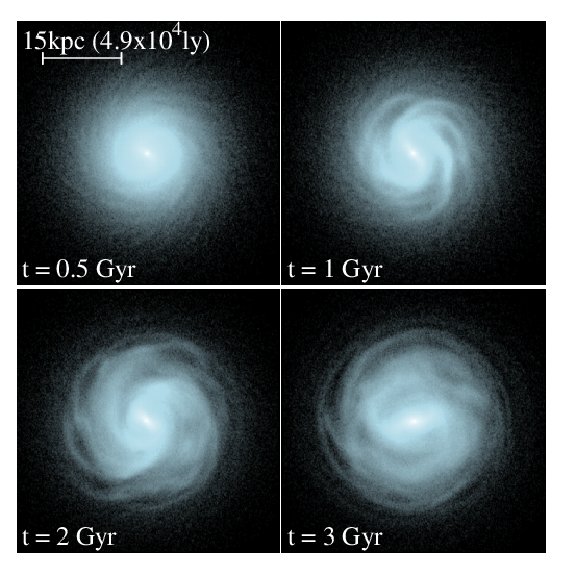
\includegraphics[width=8cm]{figure/disk.eps}
  \end{center}
  \caption{
  Face-on surface density maps of the bulge and disk.
  }
  \label{fig:evolutiondisk}
\end{figure}

Figure~\ref{fig:disk_weak} shows the measured weak-scaling
performance. We fixed the number of particles per core to 266,367 and
measured the performance for the number of cores in the range of 4096
to 663,552 on the K computer, and in the range of 32 to 2048 on
XC30. We can see that the measured efficiency and scalability are both
very good. The efficiency is more than 50\% for the entire range of
cores on the K computer. The efficiency of XC30 is a bit worse than
that of the K computer. This difference comes from the difference of
two processors. The Fujitsu processor showed higher efficiency, while
the Intel processor has 5.2 times higher peak performance per core. We
can see that the time for domain decomposition increase as we increase
the number of cores. The slope is around 2/3 as can be expected from
our current algorithm discussed in section \ref{sec:decomposition}.

%, because of the difference of SIMD vector
%length. Since the SIMD vector length on XC30 is four times longer than
%that on the K computer, the efficient usage of SIMD units on XC30 is
%more difficult than that on the K computer. We can see the increase of
%time spent for domain decomposition is slower than that of the number
%of cores. This is because that we use parallelized domain
%decomposition described in section \ref{sec:decomposition}.

Figure~\ref{fig:disk_strong} shows the measured strong-scaling
performance. We fixed the total number of particles to $550$ million
and measured the performance for 512 to 32768 cores on K computer and
256 to 2048 cores on XC30. We can also see the measured efficiency and
scalability are both very good, for the strong-scaling performance.



%The efficiency is about 50\% for the entire range of nodes.

%Figure~\ref{fig:disk_strong} shows the breakups of the measured
%strong-scaling performance. 

%Wallclock time shows slight increase for larger number of
%nodes, but this is due to the increase of the calculation cost and not
%due to the degradation of the efficiency.

%Figure~\ref{fig:disk_strong} shows the measured strong-scaling
%performance. We fixed the number of particles per node to $2.1$ million particles. We
%can see the measured efficiency and scalability are both very
%good. Efficiency is very close to 50\%, for both models and for the
%entire range of nodes. Wallclock time shows slight increase for larger
%number of nodes, but this is due to the increase of the calculation
%cost and not due to the degradation of the efficiency.

\citet{Bedorf:2014:PGT:2683593.2683600}
reported the wallclock time of 4 seconds for their 27-billion particle
simulation on the Titan system with 2048 NVIDIA Tesla K20X, with the
theoretical peak performance of 8PF (single precision, since the
single precision was used for the interaction calculation). This
corresponds to 0.8 billion particles per second per petaflops. Our
code on K computer requires 15 seconds on 16384 nodes (2PF theoretical
peak), resulting in 1 billion particles per second per
petaflops. Therefore, we can conclude that our FDPS code achieved the
performance slightly better than one of the best codes specialized to
gravitational $N$-body problem.

\begin{figure}
  \begin{center}
    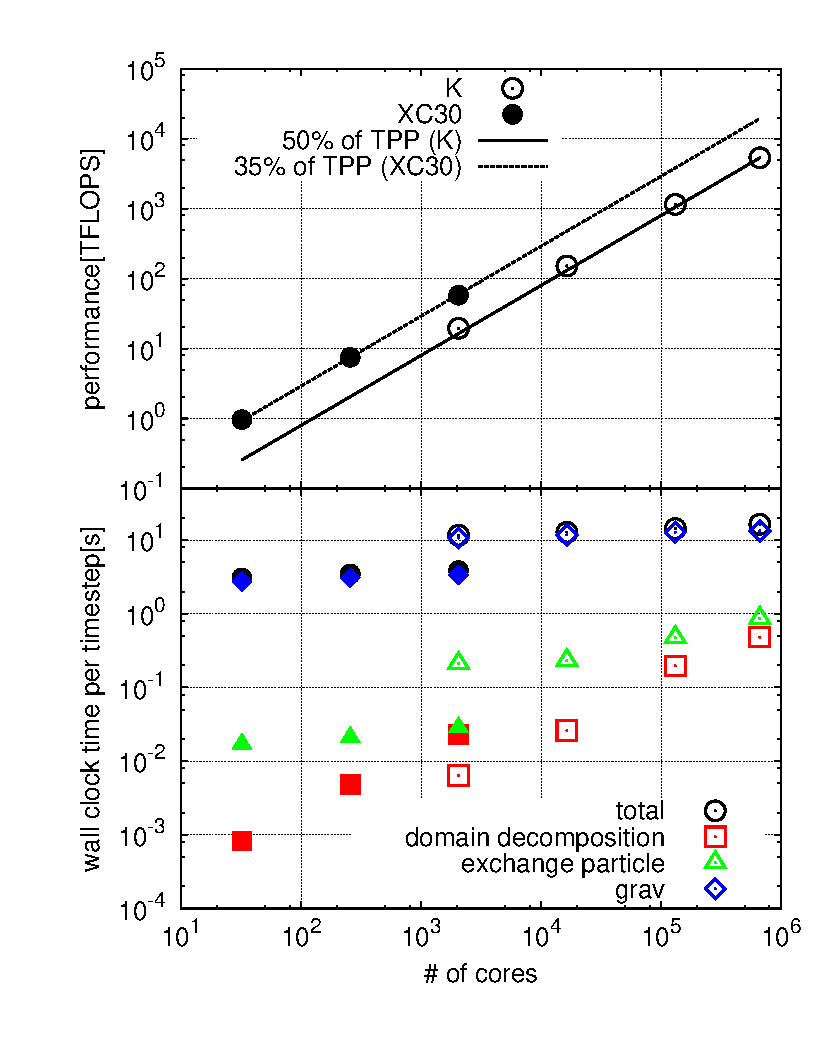
\includegraphics[width=8cm]{figure/disk_weak.eps}
  \end{center}
  \caption{
  
    Weak-scaling performance of the gravitational $N$ body code. The
    speed of the floating-point operation (top) and wallclock time per
    one timestep (bottom) are plotted as functions of the number of
    cores. Open and filled symbols indicate the performances of K
    computer and cray XC30, respectively. In the top panel, the solid
    line indicates 50\% of the theoretical peak performance of K
    computer and the dotted line indicates 35\% of the theoretical
    peak performance of XC30. In the bottom panel, time spent for the
    interaction calculation (diamond), the domain decomposition
    (square) the exchange particles (triangle) are also shown.
    
    } \label{fig:disk_weak}
\end{figure}

\begin{figure}
  \begin{center}
    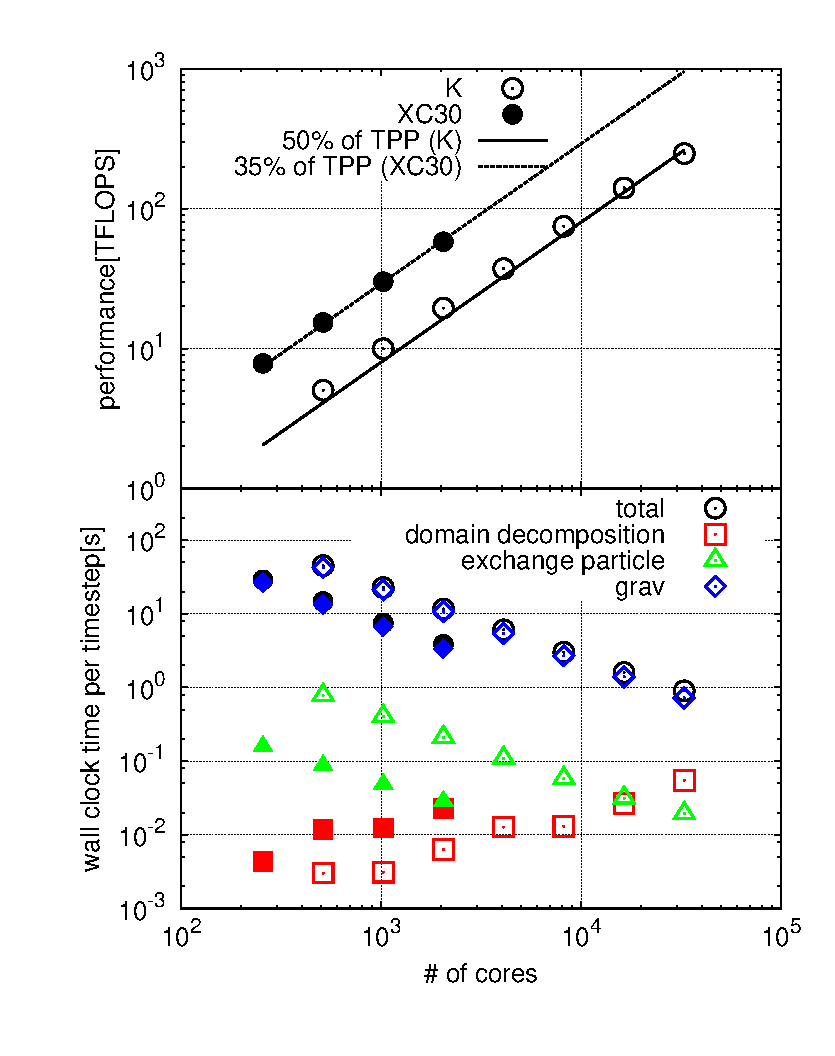
\includegraphics[width=8cm]{figure/disk_strong.eps}
  \end{center}
  \caption{
  
The same figure as figure \ref{fig:disk_weak} but for the
strong-scaling performance for 550 million particles

    }
  \label{fig:disk_strong}
\end{figure}

% LocalWords:  FDPS superparticle monopole quadrupole SIMD builtin Hernquist IC
% LocalWords:  Frenk NFW EP scalability TPP PFLOPS NVIDIA kpc axisymmetric pc
% LocalWords:  GalacticICS Gyrs timestep edorf et al petaflops Wallclock
% LocalWords:  wallclock


\subsection{Cosmological simulation}


In this section, we discuss the performance of a cosmological
simulation code implemented using FDPS. We implemented TreePM (Tree
Particle-Mesh) method and measured the performance on XC30. Our TreePM
code is based on the code developed by K. Yoshikawa. The Particle-Mesh
part of the code was developed by
\citet{Ishiyama:2012:PAN:2388996.2389003} and this code is included in
the FDPS package as an external module.

We initially place particles uniformly in a cube and gave them zero
velocity. For the calculation of the tree force , we used a monopole
only kernel with cutoff. The cutoff length of the force is three times
larger than the width of the mesh. We set $\theta$ to 0.5. For the
calculation of the mesh force, the mass density is assigned to each of
the grid points, using the triangular shaped cloud scheme and the
density profile we used is the S2 profile \citep{hockney1988computer}.

Figures \ref{fig:cosmo_weak} and \ref{fig:cosmo_strong} show the weak
and strong scaling performance, respectively. For the weak-scaling
measurement, we fixed the number of particles per process to 5.73
million and measured the performance for the number of cores in the
range of 192 to 12000 on XC30. For the strong-scaling measurements, we
fixed the total number of particles to $2048^3$ and measured the
performance for the number of cores in the range of 1536 to 12000 on
XC30. We can see that the time for the calculation of the tree force
is dominant and both of the weak and strong scalings are good except
for the very large number of cores (12000) for the strong scaling
measurement. One reason is that the scalability of the calculation of
the mesh force is not very good. Another reason is that the time for
the domain decomposition grows linearly for large number of cores,
because we did not use parallelized domain decomposition here. The
efficiency is 7\% of the theoretical peak performance. It is rather
low compared to that for the disk galaxy simulations in
section \ref{sec:diskgalaxy}. The main reason is that we use a lookup
table for the force calculation. If we evaluate the force without the
lookup table, the nominal efficiency would be much better, but the
total time would be longer.

\begin{figure}
  \begin{center}
    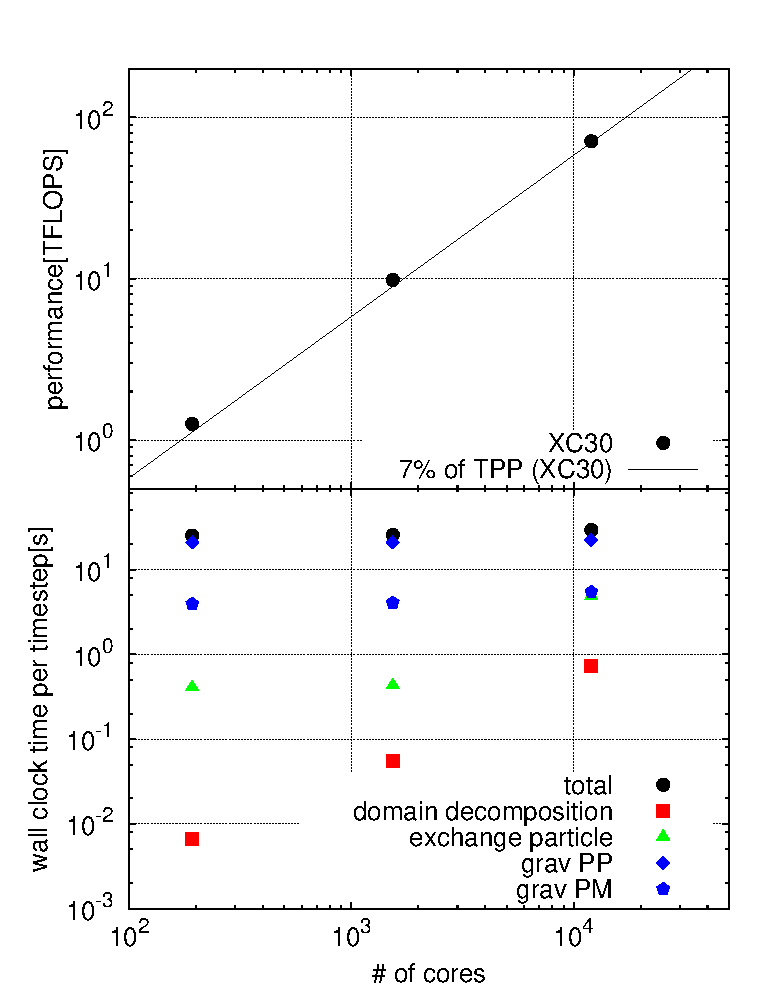
\includegraphics[width=8cm]{figure/cosmo_weak.eps}
  \end{center}
  \caption{

    Weak-scaling performance of the TreePM code. The speed of the
    floating-point operation (top) and wallclock time per one timestep
    (bottom) are plotted as functions of the number of cores. In the
    top panel, the solid line indicates 7\% of the theoretical peak
    performance of XC30. In the bottom panel, time spent for the
    Particle-Particle interaction calculation (diamond), the
    Particle-Mesh interaction (pentagon), the domain decomposition
    (square) and the exchange particles (triangle) are also shown.
    
  }
  \label{fig:cosmo_weak}
\end{figure}

\begin{figure}
  \begin{center}
    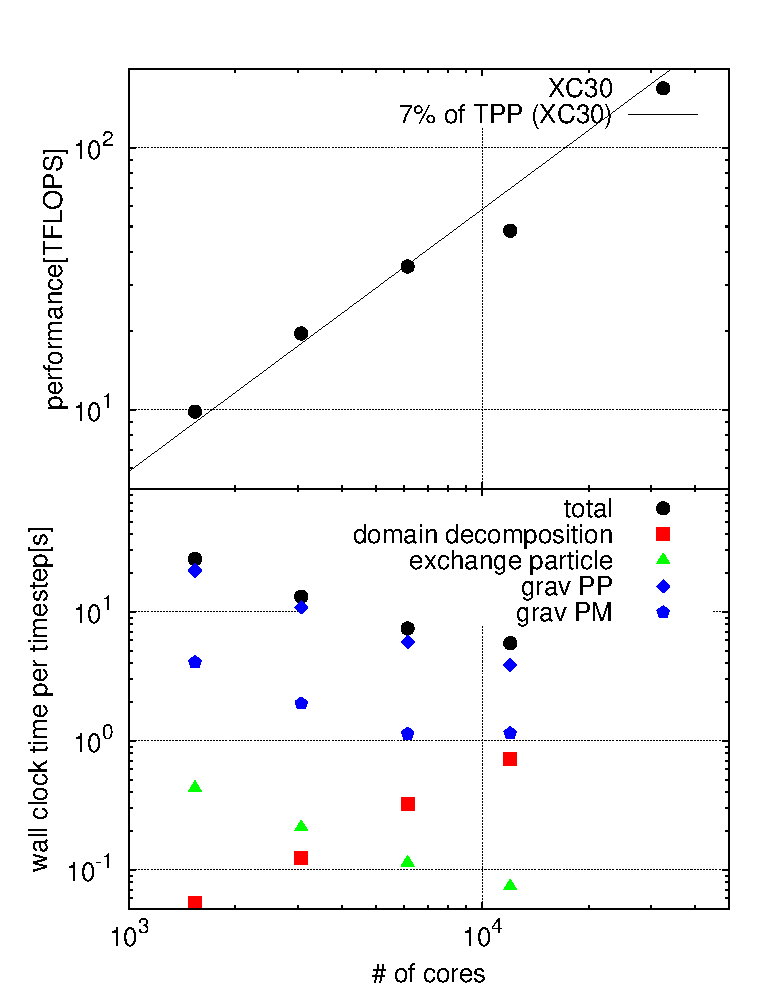
\includegraphics[width=8cm]{figure/cosmo_strong.eps}
  \end{center}
  \caption{

    The same as figure \ref{fig:cosmo_weak} but for the strong-scaling
    performance. In this case, the number of particles is $2048^3$.

  }
  \label{fig:cosmo_strong}
\end{figure}



\subsection{Giant impact simulation}

\label{sec:sph}

In this section, we discuss the performance of an SPH simulation code
with self-gravity implemented using FDPS.  Some results in this
scetion have been published in \citet{2015FDPS}.  The test problem
used is the simulation of GI. The GI
hypothesis \citep{1975Icar...24..504H, 1976LPI.....7..120C} is one of
the most popular scenarios for the formation of the Moon. The
hypothesis is as follows. About 5 billion years ago, a Mars-sized
object (hereafter, the impactor) collided with the proto-Earth
(hereafter, the target). A large amount of debris was scattered, which
first formed the debris disk and eventually the Moon. Many researchers
have performed simulations of GI, using the SPH method
\citep{1986Icar...66..515B, 2013Icar..222..200C, 2014NatGe...7..564A}.

For the gravity, we used monopole-only kernel with $\theta=0.5$. We
adopt the standard SPH scheme
\citep{1992ARA&A..30..543M, 2009NewAR..53...78R, 2010ARA&A..48..391S}
for the hydro part. Artificial viscosity is used to handle shocks
\citep{1997JCoPh.136..298M}, and 
the standard Balsara switch is used to reduce the shear viscosity
\citep{1995JCoPh.121..357B}. A kernel function we used is the Wendland $C^6$ and the cutoff radius
is 4.2 times larger than the local mean inter-particle distance. In
other words, each particle interact with about 300 particles. This
neighbor number is the appropriate for this kernel to avoid the
pairing instability \citep{2012MNRAS.425.1068D}.


%In all simulations, we set the cutoff radius to be 4.2 times larger
%than the local mean inter-particle distance. In other words, each
%particle interact with about 300 particles.

%In all GI simulations, we make three instances of
%class \texttt{TreeForForce}. One is for evaluating the density and the
%smoothing length of the kernel function for i-th particle. The second
%tree is for solving the Euler equation. In other words, we evaluate
%pressure gradient, the artificial viscosity and the Balsara switch
%with this tree.  The other tree is for gravity force.

Assuming that the target and impactor consist of granite, we adopt
equation of state of granite \citep{1986Icar...66..515B} for the
particles. For the initial condition, we assume the parabolic orbit
with the initial angular momentum 1.21 times of the current Earth-Moon
system.

%The initial conditions, such as the orbital parameters of
%the two objects, are the same as those in \citet{1986Icar...66..515B}.

%In this paper, we report the weak scaling performance with about 250k
%particles per cores. For the largest calculation, we used $1.0$
%billion particles and $4096$ nodes.

\begin{figure}
  \begin{center}
    \includegraphics[width=8cm]{figure/GI.eps}
  \end{center}
  \caption{Temperature maps of the target and impactor in the run with
  $9.9$ million particles at four different epochs. }
  \label{fig:evolutionGI}
\end{figure}

Figure~\ref{fig:evolutionGI} shows the time evolution of the target
and impactor for a run with 9.9 million particles. We can see that the
shocks are formed just after the moment of impact in both the target
and impactor ($t=2050$ sec). The shock propagates in the target, while
the impactor is completely disrupted ($t=2847$ sec) and debris are
ejected. A part of the debris falls back to the target, while the rest
will eventually form the disk and the Moon. So far, the resolution
used in the published papers have been much lower. We plan to use this
code to improve the accuracy of the GI simulations.

Figure~\ref{fig:gi_weak} and \ref{fig:gi_strong} show the measured
weak and strong scaling performance. For the weak-scaling measurement,
we fixed the number of particles per core to 20,000 and measured the
performance for the number of cores in the range of 256 to 131,072 on
the K computer. On the other hand, for the strong-scaling measurement,
we fixed the total number of particles to $39$ million and measured
the performance for the number of cores in the range of 512 to 16,384
on K computer. We can see that the performance is good even for very
large number of cores. The efficiency is about 40\% of the theoretical
peak performance. The hydro part consumes more time than the gravity
part does, mainly because the particle-particle interaction is more
complicated.

%Figure~\ref{fig:gi_strong} shows the measured strong-scaling
%performance. We fixed the total number of particles to $39$ million
%and measured the performance for number of cores in the range of 512
%to 16384 on K compute.

\begin{figure}
  \begin{center}
    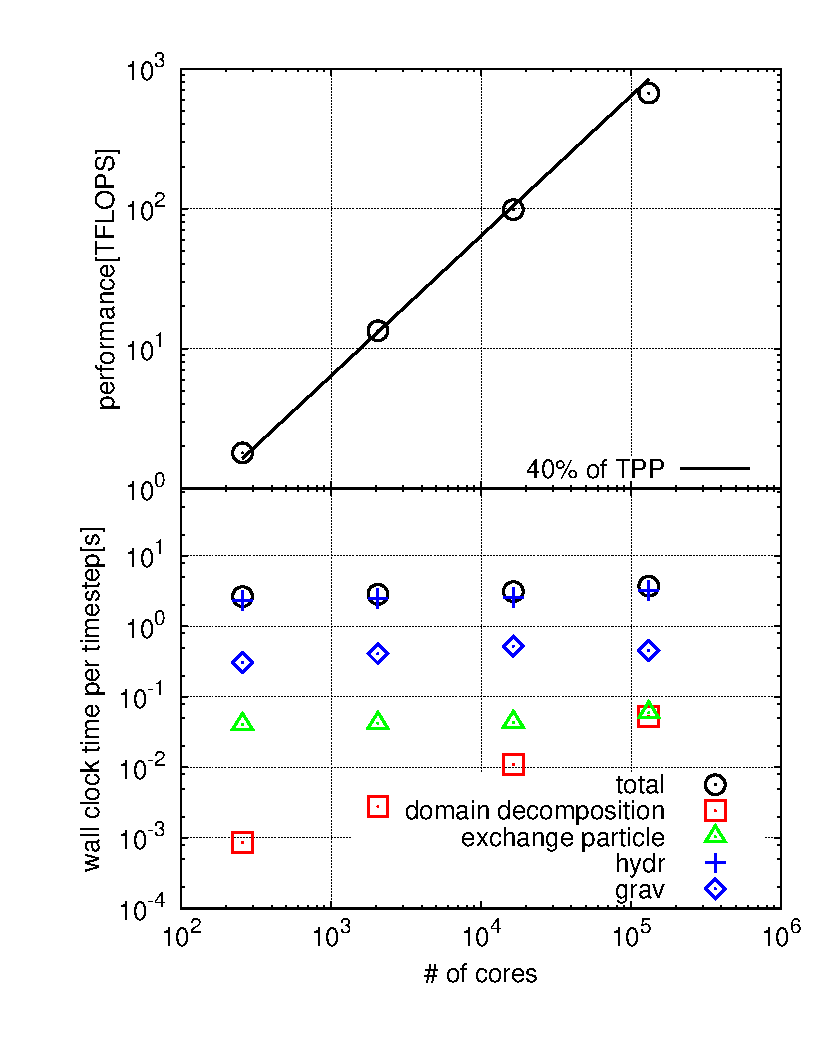
\includegraphics[width=8cm]{figure/gi_weak.eps}
  \end{center}
  \caption{

    Weak-scaling performance of the SPH code. The speed of the
    floating-point operation (top) and wallclock time per one timestep
    (bottom) are plotted as functions of the number of cores. In the
    top panel, the solid line indicates 40\% of the theoretical peak
    performance of K computer. In the bottom panel, time spent for the
    hydrodynamics calculation (cross), the gravity calculation
    (diamond), the domain decomposition (square) the exchange
    particles (triangle) are also shown.

}
  \label{fig:gi_weak}
\end{figure}

\begin{figure}
  \begin{center}
    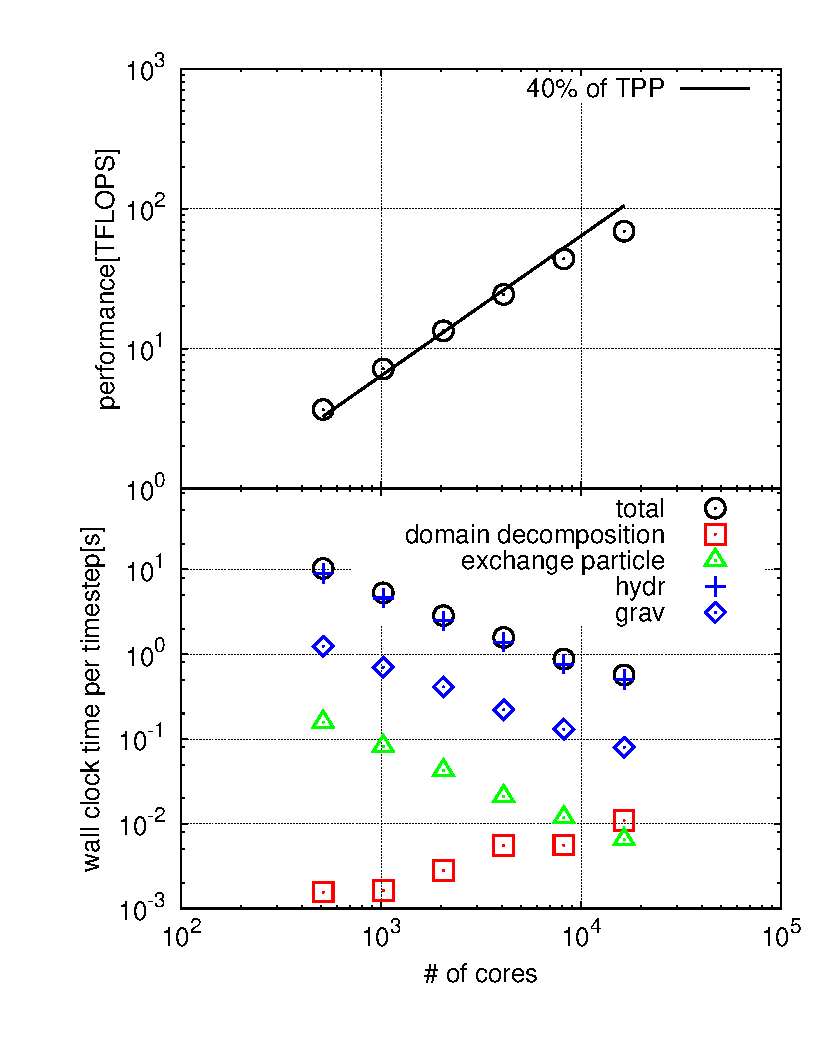
\includegraphics[width=8cm]{figure/gi_strong.eps}
  \end{center}
  \caption{

The same as figure \ref{fig:gi_weak} but for the strong-scaling
performance for $39$ million particles.

}
  \label{fig:gi_strong}
\end{figure}


%The largest number of particles used for GI simulations so far
%reported is 100 million \cite{2014LPI....45.2703T}. Unfortunately,
%performance numbers are not given. After we replace the interaction
%kernels with SIMD-optimized ones for hydrodynamics part, we believe we
%can achieve the performance not so much lower than that we achieved
%for pure gravity calculation.

% LocalWords:  SPH FDPS impactor proto Balsara rr rrr Grav Wendland SIMD

% LocalWords:  builtin Wallclock timestep wallclock monopole



\section{Performance model}
\label{sec:performancemodel}

In this section, we present the performance model of applications
implemented using FDPS. As described in section \ref{sec:user}, the
calculation of a typical application written using FDPS proceeds in
the following steps

\begin{enumerate}
  \item Update the domain decomposition and exchange particles
    accordingly (not in every timestep).
  \item  Construct the local tree structure and exchange particles and
    superparticles necessary for interaction calculation.
  \item Construct the ``global'' tree.
  \item Perform the interaction calculation.
  \item Update the physical quantities of particles using the
    calculated interactions.
\end{enumerate}

In the case of complex applications which require more than one
interaction calculations, each of the above steps, except for the
domain decomposition, may be executed more than one time per one
timestep.

For a simple application, thus, the total wallclock time per one timestep should
be expressed as
\begin{equation}
  \label{eq:totalcost}
  T_{\rm step} =  T_{\rm dc}/n_{\rm dc}
               + T_{\rm lt}
               + T_{\rm exch}
               + T_{\rm icalc}
               + T_{\rm misc},
\end{equation}
where   $T_{\rm dc}$, $T_{\rm lt}$, $T_{\rm exch}$,
$T_{\rm icalc}$, and $T_{\rm misc}$ are the times for
domain composition and particle exchange, local tree construction,
exchange of particles and superparticles for interaction calculation,
interaction calculation, and other calculations such as particle
update, respectively. The term $n_{\rm dc}$ is the interval at which
the domain decomposition is performed.

In the following, we first construct the model for the communication
time. Then we construct models for each term of the right hand side of
equation~\ref{eq:totalcost}, and finally we compare the model with the
actual measurement presented in section
\ref{sec:total_time}.

\subsection{Communication model}
\label{sec:comm_model}

What ultimately determines the efficiency of a calculation performed
on a large-scale parallel machine is the communication overhead. Thus,
it is very important to understand what types of communication would
take what amount of time on actual hardware. In this section, we
summarize the characteristics of the communication performance of K
computer.

In FDPS, almost all communications are through the use of collective
communications, such as {\tt MPI\_Allreduce}, {\tt MPI\_Alltoall}, and
{\tt MPI\_Alltoallv}. However, measurement of the performance of these
routines for uniform message length is not enough, since the amount of
data to be transferred between processes generally depends on the
physical distance between domains assigned to those
processes. Therefore, we first present the timing results for simple
point-to-point communication, and then for collective communications.

Figure \ref{fig:pingpong} shows the elapsed time as the function of
the message length, for point-to-point communication between
``neighboring'' processes. In the case of K computer, we used
three-dimensional node allocation, so that ``neighboring'' processes
are actually close to each other in its torus network.

%For Cray XC30 we let the system to allocate nodes in its default
%mode.

We can see that the elapsed time can be fitted reasonably well as
\begin{equation}
\label{eq:Tp2p}
  T_{\rm p2p} = T_{\rm p2p,startup} + n_{\rm word}T_{\rm p2p,word},
\end{equation}
where $T_{\rm p2p,startup}$ is the startup time which is independent
of the message length and $T_{\rm p2p,word}$ is the time to transfer
one byte of message. Here, $n_{\rm word}$ is the length of the message
in units of bytes. On K computer, $T_{\rm p2p,startup}$ is 0.0101 ms
and $T_{\rm p2p,word}$ is $2.11 \times 10^{-7}$ ms per byte. For a
short message, there is a rather big discrepancy between the analytic
model and measured points, because for short messages K computer used
several different algorithms.


\begin{figure}
  \begin{center}
    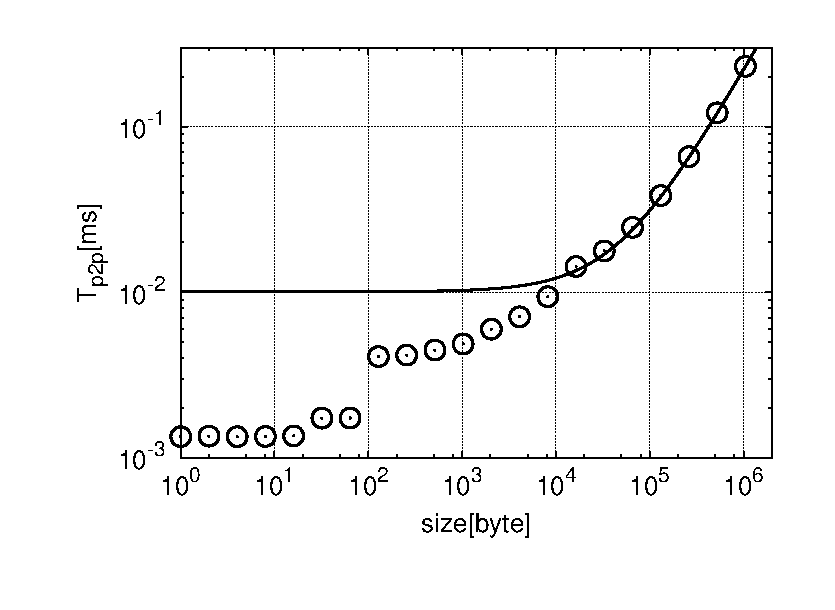
\includegraphics[width=8cm]{figure/pingpong.eps}
  \end{center}
  \caption{
  
  Elapsed time for point-to-point communication as a function of size
  of message measured on K computer.

}
  \label{fig:pingpong}
\end{figure}



Figure \ref{fig:group_comm_a2a} shows the elapsed times for {\tt
MPI\_Alltoallv}. The number of processes $n_p$ is 32 to 2048. They are
again modeled by the simple form
\begin{equation}
\label{eq:wtime_group_comm}
  T_{\rm alltoallv} = T_{\rm alltoallv,\rm startup} + n_{\rm word}T_{\rm alltoallv,\rm word}, 
\end{equation}
where $T_{\rm \rm alltoallv,\rm startup}$ is the startup time and
$T_{\rm alltoallv,\rm word}$ is the time to transfer one byte of message.
We list these values in table \ref{table:alltoallv}.

\begin{table}
\caption{Time coefficients in equation (\ref{eq:wtime_group_comm})}
\begin{tabular}{|l|l|l|l|} \hline
                  & $n_p=32$ & $n_p=256$ & $n_p=2048$ \\ \hline
$T_{\rm alltoallv,startup}$ [ms] & 0.103 & 0.460 & 2.87 \\
$T_{\rm alltoallv,word}$ [ms/byte] & $8.25\times 10^{-6}$  & $9.13\times 10^{-5}$ & $1.32\times 10^{-3}$  \\ \hline
\end{tabular}
\label{table:alltoallv}
\end{table}


%In table \ref{table:domain_decomposition} we list these time coefficients.
%We can see that the agreement is reasonable. In
%table \ref{table:domain_decomposition} we list the values of these
%time constants.

The coefficients themselves in equation (\ref{eq:wtime_group_comm})
depend on the number of MPI processes $n_p$, as shown in
figures \ref{fig:group_comm_a2a_2}. They are modeled as
\begin{eqnarray}
\label{eq:alltoallv}
  T_{\rm alltoallv,startup} &=& \tau_{\rm alltoallv,startup} n_p, \\
  T_{\rm alltoallv,word} &=& \tau_{\rm alltoallv,word} n_p^{4/3}.
\end{eqnarray}
Here we assume that the speed to transfer message using {\tt
MPI\_Alltoallv} is limited to the bisection bandwidth of the system.
Under this assumption, $T_{\rm alltoallv,word}$ should be proportional
to $n_p^{4/3}$.  To estimate $\tau_{\rm alltoallv,startup}$ and
$\tau_{\rm alltoallv,word}$, we use measurements for message sizes of
8 bytes and 32k bytes. In K computer, we found that $\tau_{\rm
alltoallv,startup}$ is $0.00166$ ms and $\tau_{\rm alltoallv,word}$ is
$1.11 \times 10^{-7}$ ms per byte. If {\tt MPI\_Alltoallv} is limited
to the bisection bandwidth in K computer, $\tau_{\rm alltoallv,word}$
would be $5 \times 10^{-8}$ ms per byte. We can see that the actual
performance of {\tt MPI\_Alltoallv} on K computer is quite good.


%The two fittings to $T_{\rm alltoallv,startup}$ and $\tau_{\rm
%alltoallv,word}$ are reasonably well.

\begin{figure}
  \begin{center} 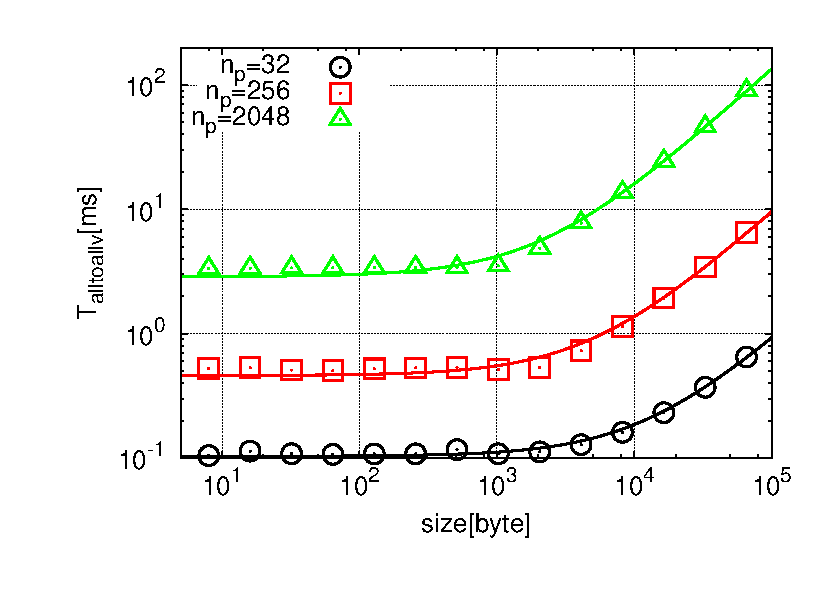
\includegraphics[width=8cm]{figure/comm/group_comm_a2a.eps}
  \end{center}
  \caption{
  
    Elapsed time of {\tt MPI\_Alltoallv} as a function of message size
    measured on K computer.

}
\label{fig:group_comm_a2a}
\end{figure}

\begin{figure}
  \begin{center}
  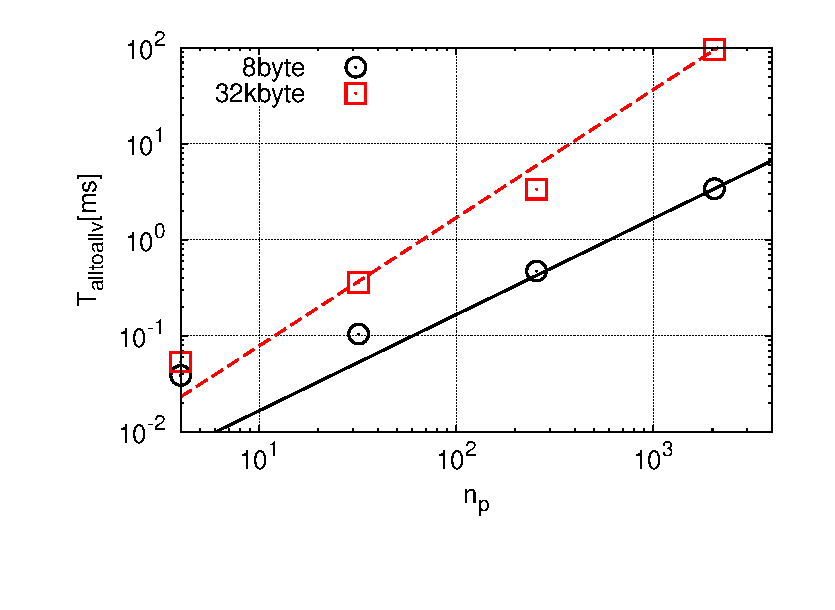
\includegraphics[width=8cm]{figure/comm/group_comm_a2a_2.eps}
  \end{center}
  \caption{
  
    Elapsed time of {\tt MPI\_Alltoallv} to send messeage of 8 bytes
    (circles) and 32k bytes (squares) as a function of the number of
    processes measured on K computer. Solid and dashed curves indicate
    the results for the message size of 8 bytes and 32k bytes,
    respectively.
    
} \label{fig:group_comm_a2a_2}
\end{figure}

%\begin{eqnarray}
%  T_{\rm type,startup} &=& \tau_{\rm type,startup} n_p \\
%  T_{\rm type,word} &=& \tau_{\rm type,word} n_p^{\alpha_{\rm type}}.
%\end{eqnarray}
%$T_{\rm alltoallv,word}$ and $T_{\rm allgatherv,word}$ are determined
%by the bisection and injection bandwidth. Thus $\alpha_{\rm
%alltoallv}$ is $4/3$ and $\alpha_{\rm allgatherv}$ is unity.

%Fitting the equations \ref{eq:alltoallv}, $\tau_{\rm
%alltoallv,startup}$ is $0.00166$ ms and $\tau_{\rm alltoallv,word}$ is
%0.00364 ms.


\subsection{Domain decomposition}

For the hierarchical domain decomposition method described in
section \ref{sec:decomposition}, the calculation time is expressed as

\begin{equation}
  \label{eq:dccost}
  T_{\rm dc} = T_{\rm dc,gather}
            +   T_{\rm dc,sort}
            +   T_{\rm dc,exch}
            +   T_{\rm dc,misc},
\end{equation}
where $T_{\rm dc,gather}$ is the time for the $(i,0,0)$ process to
collect sample particles, $T_{\rm dc,sort}$ is the time to sort sample
particles on the $(i,0,0)$ process, $T_{\rm dc,exch}$ is the time to
exchange particles after the new domains are determined, and $T_{\rm
dc,misc}$ is the time for remaining procedures such as initial
exchange of samples in $x$ direction, exchange of sample particles and
domain boundaries in $x$ direction, and broadcasting of the domain
boundaries in $y$-$z$ planes.

On the machines we so far tested, $T_{\rm dc,gather}$ and $T_{\rm
  dc,misc}$ are much smaller than $T_{\rm dc,sort}$ and $T_{\rm
  dc,exch}$. Therefore we consider these two terms only.

First, we consider the time to sort sample particles. Since we use the
quick sort, the term $T_{\rm dc,sort}$ is expressed as
%\begin{eqnarray}
%T_{\rm dc,sort} &=& \tau_{\rm qsort} \left[ 2n_{\rm smp} n_y n_z {\rm log} (n_{\rm smp} n_y n_z) + n_y n_{\rm smp} n_z {\rm log} (n_{\rm smp} n_z) \right], \\ 
%             &\sim& \tau_{\rm qsort} \left[ 2n_{\rm smp} n_p^{2/3} {\rm log} (n_{\rm smp} n_p^{2/3}) + n_p^{2/3} n_{\rm smp} {\rm log} (n_{\rm smp} n_p^{1/3}) \right],
%\end{eqnarray}
\begin{eqnarray}
T_{\rm dc,sort} &=& \tau_{\rm sort} \left[ 2n_{\rm smp} n_y n_z {\rm log} (n_{\rm smp} n_y n_z) + n_y n_{\rm smp} n_z {\rm log} (n_{\rm smp} n_z) \right] \\ 
             &\sim& \tau_{\rm dc,sort} n_{\rm smp}n_p^{2/3},
\end{eqnarray}
where $n_{\rm smp}$ is the average number of sample particles per
process, and $n_x$, $n_y$ and $n_z$ are the numbers of processes in x,
$y$ and $z$ direction. Here, $\tau_{\rm dc,sort} \sim {\rm log}(n_{\rm
smp}^3n_p^{5/3})\tau_{\rm sort}$. The first term expresses the time to
sort samples in $y$-$z$ planes with respect to $x$ and $y$
directions. The second term expresses that time to sort samples
respect to $z$ direction.

In order to model $T_{\rm dc,exch}$, we need to model the number of
particles which moves from one domain to another. This number would
depend on various factors, in particular the nature of the system we
consider. For example, if we are calculating the early phase of the
cosmological structure formation, particles do not move much in a
single timestep, and thus the number of particles moved between
domains is small. On the other hand, if we are calculating single
virialized self-gravitating system, particles move a relatively large
distances (comparable to average interparticle distance) in a single
timestep. In this case, if one process contains $n$ particles, half of
particles in the ``surface'' of the domain might migrate in and out
the domain. Thus, $O(n^{2/3})$ particles could be exchanged in this
case.

Figures \ref{fig:domain_decomposition_sort}, \ref{fig:domain_decomposition_exch}
and \ref{fig:domain_decomposition} show the elapsed time for sorting
samples, exchanging samples, and domain decomposition for the case of
disk galaxy simulations in the case of $n_{\rm smp}=500$ and $n \sim
5.3 \times 10^5$. We also plot the analytic models given by
\begin{eqnarray}
\label{eq:ddfit}
  T_{\rm dc} &\sim& T_{\rm dc,sort} + T_{\rm dc,exch} \\
             &=& \tau_{\rm dc,sort} n_{\rm smp} n_p^{2/3}
                 + \tau_{\rm dc,exch} \sigma \Delta t / \left<r\right> n^{2/3} b_p,
\end{eqnarray}
where $\tau_{\rm dc,sort}$ and $\tau_{\rm dc,exch}$ are the execution
time for sorting one particle and for exchanging one particle
respectively, $\sigma$ is the typical velocity of particles, $\Delta
t$ is the timestep and $\left<r\right>$ is the average interparticle
distance. For simplicity we ignore weak log term in $T_{\rm dc,sort}$
. On K computer, $\tau_{\rm dc,sort} = 2.67\times 10^{-7}$ second and
$\tau_{\rm dc,exch} = 1.42\times 10^{-7}$ second per byte. Note that
$\tau_{\rm dc,exch} \sim 672 T_{\rm p2p,word}$.

In figure \ref{fig:domain_decomposition_exch}, for small $n_p$, the
analytic model gives the value about 2 times smaller than the measured
point. This is because the measured values include not only the time
to exchange particles but also the time to determine appropriate
processes to send particles, while the analytic model includes only
the time to exchange particles. For small $n_p$, the time to determine
the appropriate process is not negligible, and therefor the analytic
model gives an underestimate.

%From figure \ref{fig:domain_decomposition_exch}, we can see that the
%left point is shifted upward from the fitted curve. This is because we
%used the least squares fitting and the right and center points are
%more highly weighted than the left one. In addition, we assumed that
%the particles are uniformly distributed, but in the simulation, we
%used the disk galaxy model (with high density contrast). The
%difference between the performance model and the simulation for this
%part is larger for smaller number of processes, because each
%computational domain has larger density contrast. Thus the left point
%is a bit far from the fitted curve.

%Note that $\tau_{\rm dc,sort} \sim {\rm log}(n_{\rm
%smp}^3n_p^{5/3})\tau_{\rm qsort}$.

%On K computer, $\tau_{\rm dc,sort} = 1.56\times 10^{-4}$ s and
%$\tau_{\rm dc,exch} = 5.53\times 10^{-5}$ s. Note that
%Figure \ref{fig:domain_decomposition} shows $T_{\rm dc}$ measured in
%K computer and its fitting curve using \ref{eq:ddfit} against the
%number of processes, in the case of $n_{\rm smp}=500$ and $n \sim
%5.3 \times 10^5$. In this case, we use $\tau_{\rm dc,sort} =
%1.56\times 10^{-4}$ ms and $\tau_{\rm dc,exch} = 8.65\times 10^{-7}$
%ms.

\begin{figure}
  \begin{center}
    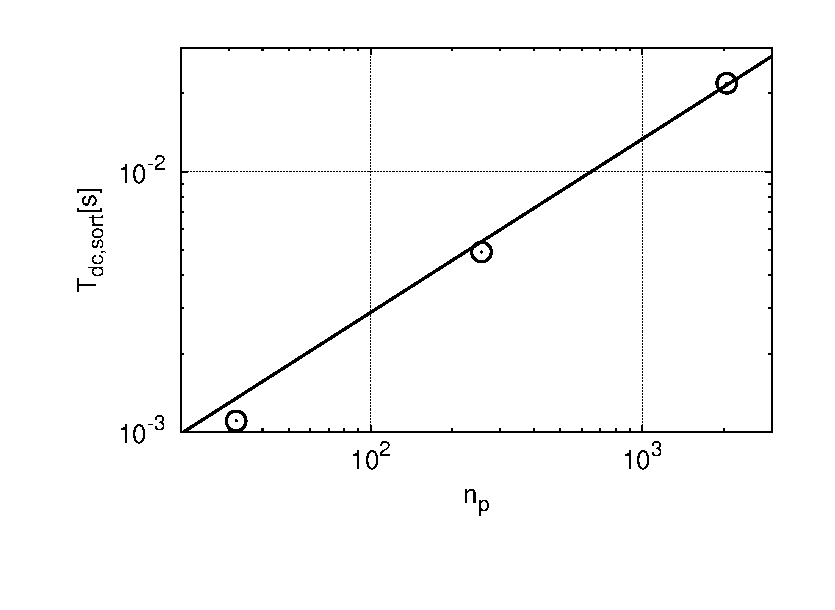
\includegraphics[width=8cm]{figure/performance/domain_decomposition_sort.eps}
  \end{center}
  \caption{

Measured $T_{\rm dc,sort}$ and its analytic model as a function of
$n_p$, in the case of $n_{\rm smp}=500$ and $n \sim 5.3 \times 10^5$.

    }
  \label{fig:domain_decomposition_sort}
\end{figure}

\begin{figure}
  \begin{center}
    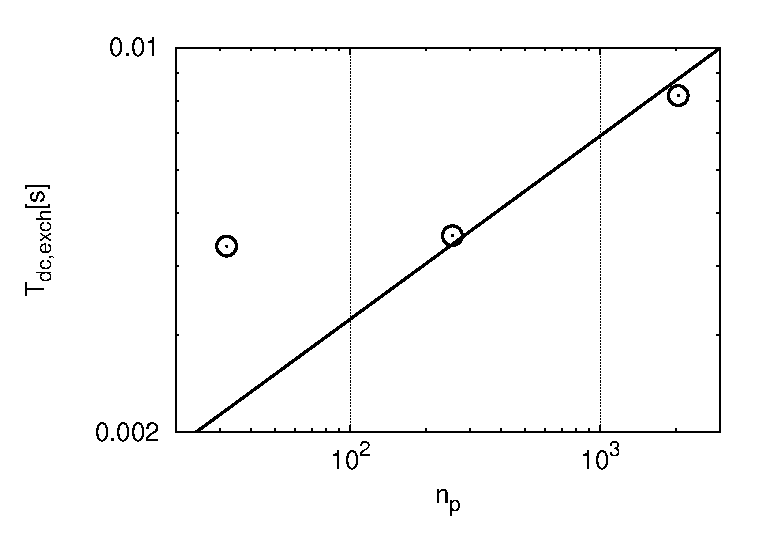
\includegraphics[width=8cm]{figure/performance/domain_decomposition_exch.eps}
  \end{center}
  \caption{

Measured $T_{\rm dc,exch}$ and its analytic model as a function of $n_p$, in
the case of $n_{\rm smp}=500$ and $n \sim 5.3 \times 10^5$.

    }
  \label{fig:domain_decomposition_exch}
\end{figure}

\begin{figure}
  \begin{center}
    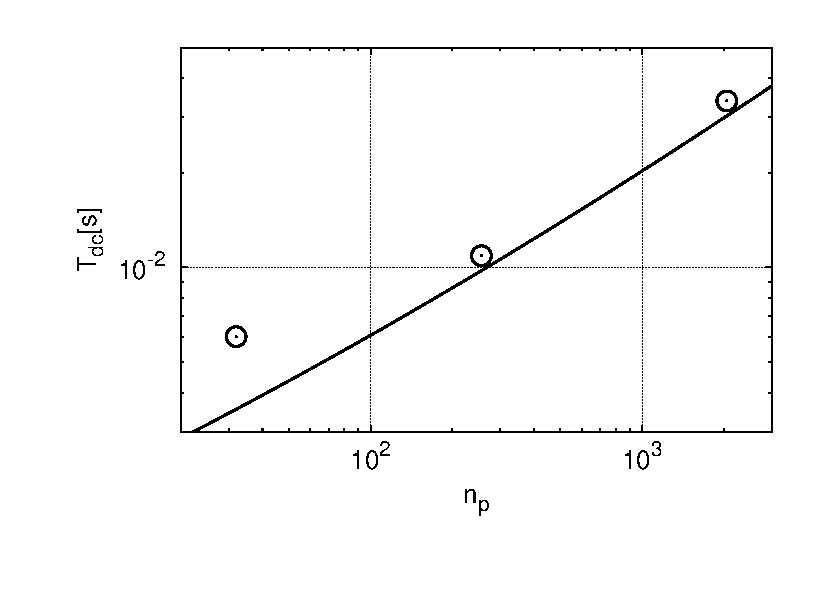
\includegraphics[width=8cm]{figure/performance/domain_decomposition.eps}
  \end{center}
  \caption{

Measured $T_{\rm dc}$ and its analytic model as a function of $n_p$,
in the case of $n_{\rm smp}=500$ and $n \sim 5.3 \times 10^5$.

    }
  \label{fig:domain_decomposition}
\end{figure}

The analysis above, however, indicates that $T_{\rm dc,exch}$ is, even
when it is relatively large, still much smaller than $T_{\rm exch}$,
which is the time to exchange particles and superparticles for
interaction calculation (see section \ref{sec:exchnage_list}).

\subsection{Tree construction}

Theoretically, the cost of tree construction is $O(n{\rm log}n)$, and
of the same order as the interaction calculations itself. However, in
our current implementation, the interaction calculation is much more
expensive, independent of target architecture and the type of the
interaction. Thus we ignore the time for the tree constructions.


\subsection{Exchange of particles and superparticles}
\label{sec:exchnage_list}

For the exchange of particles and superparticles, in the current
implementation of FDPS, first each node constructs the list of
particles and superparticles (hereafter the exchange list) to be sent
to all other nodes, and then data are exchanged through a single call
to {\tt MPI\_Alltoallv}. The way the exchange list is constructed
depends on the force calculation mode. In the case of long-range
forces, usual tree traversal with a fixed opening angle $\theta$ is
performed. For the short-range forces, the procedure used depends on
the subtypes of the interaction. In the case of fixed or $j$-dependent
cutoff, the exchange list for a node can be constructed by a single
traversal of the local tree. On the other hand, for $i$-dependent or
symmetric cutoff, first each node constructs the $j$-dependent
exchange lists and sends them to all other nodes. Each node then
constructs the $i$-dependent exchange lists and sends them again.

The time for the construction and exchange of exchange list is thus
given by
\begin{equation}
  T_{\rm exch} = k_{\rm type}(T_{\rm exch,const}+T_{\rm exch,comm}).
  \label{eq:exchangecost}
\end{equation}

Here, $k_{\rm type}$ is an coefficient which is unity for fixed and
$j$-dependent cutoffs and two for other cutoffs. Strictly speaking,
the communication cost does not double for $i$-dependent or symmetric
cutoffs, since we send only particles which were not sent in the first
step. However, for simplicity we use $k=2$ for both calculation and
communication.

The two terms in equation (\ref{eq:exchangecost}) are then
approximated as
\begin{eqnarray}
  T_{\rm exch,const} &=& \tau_{\rm exch,const} n_{\rm exch,list}, \label{eq:exchange} \\
  T_{\rm exch,comm}(n_{\rm msg}) &=&  T_{\rm alltoallv}\left( n_{\rm exch,list}/n_{p} b_p \right), \label{eq:exchange_comm}
\end{eqnarray}

where $n_{\rm exch,list}$ is the average length of the exchange list
and $\tau_{\rm exch,const}$ is the execution time for constructing one
exchange list.  Figures \ref{fig:exchangeLET_nlist-wtime_const}
and \ref{fig:exchangeLET_nlist-wtime_exch} show the execution time for
constructing and exchanging the exchange list against the average
length of the list. Here, $b_p=48$ bytes for both short and long-range
interactions. From figure \ref{fig:exchangeLET_nlist-wtime_const}, we
can see that the elapsed time can be fitted well by equation
(\ref{eq:exchange}).  Here $\tau_{\rm exch,const}$ is $1.12 \times
10^{-7}$ second for long-range interaction and $2.31 \times 10^{-7}$
second for short-range interaction.

From figure \ref{fig:exchangeLET_nlist-wtime_exch}, we can see a large
discrepancy between measured points and the curves predicted from
equation (\ref{eq:exchange_comm}). In the measurement of the
performance of ${\tt MPI\_Alltoallv}$ in section \ref{sec:comm_model},
we used uniform message length across all processes. In actual use in
exchange particles, the length of the message is not
uniform. Neighboring processes generally exchange large messages,
while distant processes exchange short message. For such cases,
theoretically, communication speed measured in terms of average
message length should be faster. In practice, however, we observed a
serious degradation of performance. This degradation seems to imply
that the current implementation of ${\tt MPI\_Alltoallv}$ is
suboptimal for non-uniform message size.

\begin{figure}
  \begin{center}
    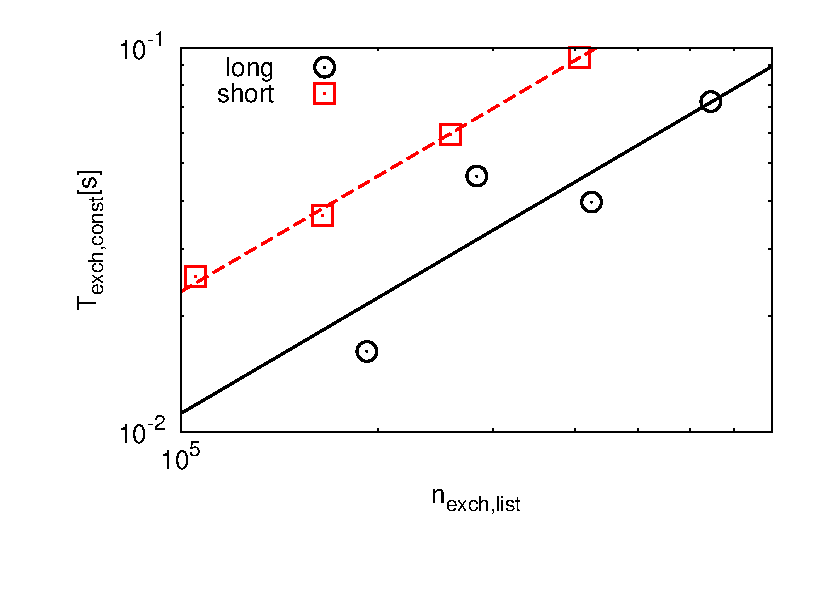
\includegraphics[width=8cm]{figure/performance/exchangeLET_nlist-wtime_const.eps}
  \end{center}
  \caption{
  
Time for the construction of the exchange list plotted against the
average length of the list, for the case of $n_p=2048$ and $n \sim
2.7 \times 10^5, 5.3 \times 10^5, 1.1 \times 10^6, 2.1 \times
10^6$. Circles and squares indicate the results for long-range and
short-range force, respectively. Solid and dashed curves are analytic
models [equation (\ref{eq:exchange})].

    }
  \label{fig:exchangeLET_nlist-wtime_const}
\end{figure}

\begin{figure}
  \begin{center}
    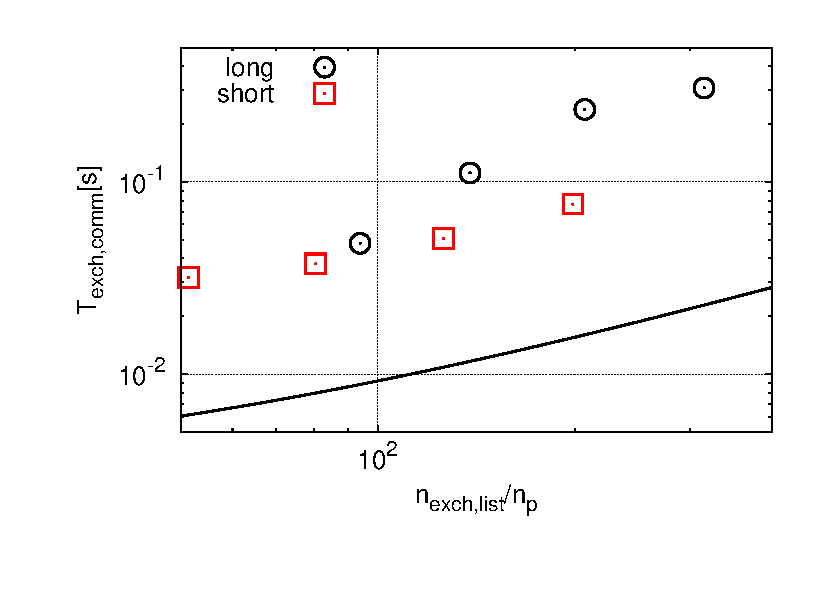
\includegraphics[width=8cm]{figure/performance/exchangeLET_nlist-wtime_exch.eps}
  \end{center}
  \caption{

Time for the communication of the exchange list against the average
length of the list per process, for the case of $n_p=2048$ and $n \sim
2.7 \times 10^5, 5.3 \times 10^5, 1.1 \times 10^6, 2.1 \times
10^6$. Circles and squares indicate the results for long-range and
short-range force, respectively. The curve is predicted from
equation (\ref{eq:exchange}).

    }
  \label{fig:exchangeLET_nlist-wtime_exch}
\end{figure}

In the following, we estimate $n_{\rm exch,list}$. If we consider a
rather idealized case, in which all domains are cubes containing $n$
particles, the total length of the exchange lists for one domain can
approximately be given by
\begin{equation}
\label{eq:n_list_long}
  n_{\rm exch,list} \sim \frac{14n^{2/3}}{\theta} + \frac{21\pi n^{1/3}}{\theta^2} + \frac{28\pi}{3\theta^3} {\rm log_2} \left\{ \frac{\theta}{2.8}\left[\left(nn_p\right)^{1/3} - n^{1/3}\right] \right\},
\end{equation}
for the case of long-range interactions and
\begin{equation}
\label{eq:n_list_short}
  n_{\rm exch,list} \sim \left( n^{1/3}-1+2\frac{r_{\rm cut}}{\left<r\right>} \right)^3-n,
\end{equation}
for the case of short-range interactions, where $r_{\rm cut}$ is the
average cutoff length and and $\left<r\right>$ is the average
interparticle distance. In this section we set $r_{\rm cut}$ so that
the number of particles in the neighbor sphere is to be 100. In other
words, $r_{\rm cut} \sim 3\left<r\right>$.

% and $n_{\rm ngb}$ is the number of the
%particles in the sphere with a radius of $r_{\rm cut}$.

In figure \ref{fig:exchangeLET_nlist-nsend}, we plot the list length
for short and long interactions against the average number of
particles. The rough estimate of equations (\ref{eq:n_list_long}) and
(\ref{eq:n_list_short}) agree very well with the measurements.

%Two curves are from
%equation \ref{eq:n_list_long} and \ref{eq:n_list_short}.

\begin{figure}
  \begin{center}
    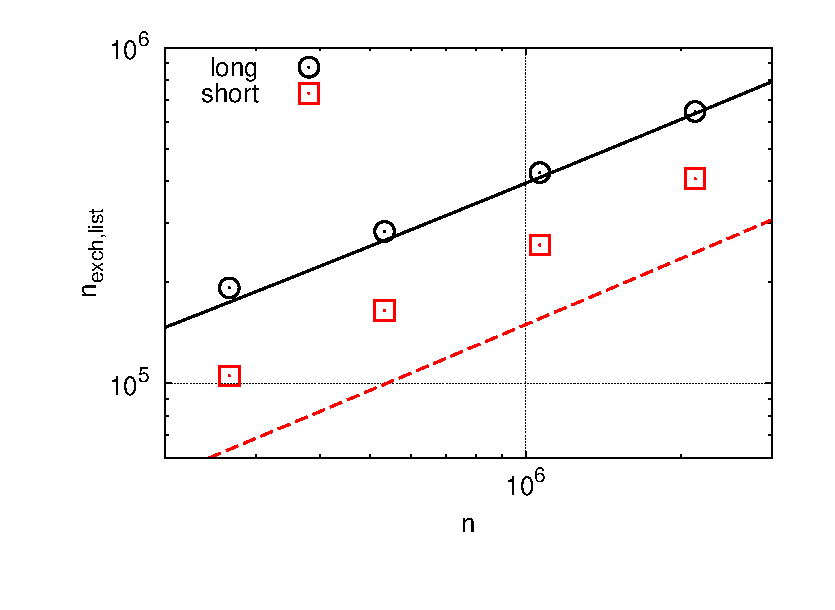
\includegraphics[width=8cm]{figure/performance/exchangeLET_n-nsend.eps}
  \end{center}
  \caption{
  
The average length of the exchange lists for long-range interaction
(circles) and for short-range interaction (squares) as a function of
$n$, in the case of $\theta=0.4$ and $n_P=2048$. Solid and dashed
curves are predicted from equations (\ref{eq:n_list_long}) and
(\ref{eq:n_list_short}), respectively.

    }
  \label{fig:exchangeLET_nlist-nsend}
\end{figure}


\subsection{Tree traverse and interaction calculation}

The time for the force calculation is given by
\begin{equation}
T_{\rm icalc} = T_{\rm icalc,force} + T_{\rm icalc,const},
\end{equation}
where $T_{\rm icalc,force}$ and $T_{\rm icalc,const}$ are the time for
the force calculations for all particles and the tree traverses for
all interaction lists, respectively.

$T_{\rm icalc,force}$ and $T_{\rm icalc,const}$ are expressed as
\begin{eqnarray}
T_{\rm icalc,const} &=& \tau_{\rm icalc,const} n n_{\rm icalc,list} / n_{\rm grp}, \label{eq:wtime_force} \\
T_{\rm icalc,force}  &=& \tau_{\rm icalc,force} n n_{\rm icalc,list},
\end{eqnarray}
where $n_{\rm icalc,list}$ is the average length of the interaction
list, $n_{\rm grp}$ is the number of $i$ particle groups for modified
tree algorithms by \citet{1990JCoPh..87..161B}, $\tau_{\rm
icalc,force}$ and $\tau_{\rm icalc,const}$ are the time for one force
calculation and for constructing one interaction list.  In
figure \ref{fig:interaction_calc_nwalk-wtime}, we plot the time for
the construction of the interaction list as a function of $n_{\rm
grp}$. On K computer, $\tau_{\rm icalc,const}$ are $3.72\times
10^{-8}$ second for the long-range force and $6.59\times 10^{-8}$
second for the short-range force.

\begin{figure}
  \begin{center}
    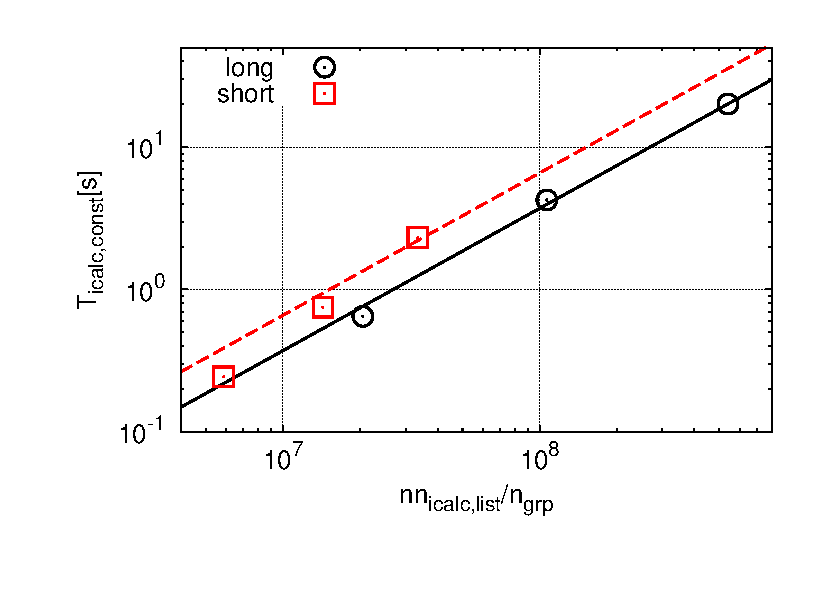
\includegraphics[width=8cm]{figure/performance/interaction_calc_nwalk-wtime.eps}
  \end{center}
  \caption{

Time for the construction of the interaction list for long-range force
(circles) and short-range force (squares), for the case of $n \sim
5.3 \times 10^5$ and $\theta = 0.4$. Solid and dashed curves are the
analytic models for long-rage and short range forces, respectively
[equation (\ref{eq:wtime_force})].

    }
  \label{fig:interaction_calc_nwalk-wtime}
\end{figure}

The length of the interaction list is given by
\begin{equation}
\label{eq:nlist_long}
  n_{\rm icalc,list} \sim n_{\rm grp} + \frac{14n_{\rm grp}^{2/3}}{\theta} + \frac{21\pi n_{\rm grp}^{1/3}}{\theta^2} + \frac{28\pi}{3\theta^3} {\rm log_2} \left[ \frac{\theta}{2.8}\left\{\left(nn_p\right)^{1/3} - n_{\rm grp}^{1/3}\right\}\right]
\end{equation}
for the case of long-range interactions and
\begin{equation}
\label{eq:nlist_short}
  n_{\rm icalc,list} \sim \left( n_{\rm grp}^{1/3}-1+2\frac{r_{\rm cut}}{\left<r\right>} \right)^3,
\end{equation}
for the case of short-range interactions.

In figure \ref{fig:interaction_calc_ng-nlist}, we plot the length of
the interactions lists for long-range force and short-range force. We
can see that the length of the interaction lists can be fitted
reasonably well.

\begin{figure}
  \begin{center}
    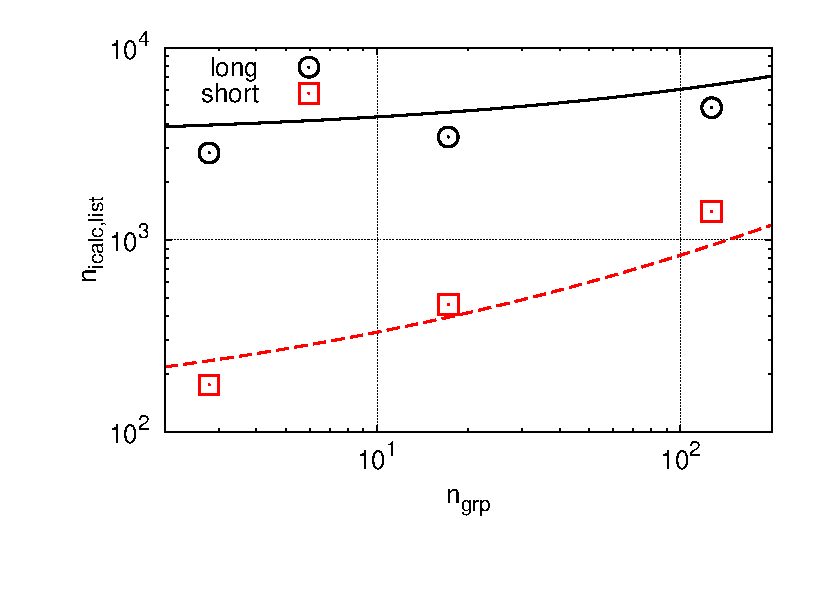
\includegraphics[width=8cm]{figure/performance/interaction_calc_ng-nlist.eps}
  \end{center}
  \caption{

The average length of the interaction list for long-range force
(circles) and short-range force (squares), for the case of $n \sim
5.3 \times 10^5$ and $\theta = 0.4$. Solid and dashed curves are
analytic models for long-range [equation (\ref{eq:nlist_long})] and
short-range [equation (\ref{eq:nlist_short})] forces.

    }
  \label{fig:interaction_calc_ng-nlist}
\end{figure}

In the following, we discuss the time for the force calculation.  The
time for the force calculation for one particle pair $\tau_{\rm
icalc,force}$ has different values for different kinds of
interactions.  We plot $\tau_{\rm icalc,force}$ against $n_{\rm
icalc,list}$ for various $n_{\rm grp}$ in
figure \ref{fig:calc_force}. We can see that for larger $n_{\rm grp}$,
$\tau_{\rm icalc,force}$ becomes smaller. However, from equation
(\ref{eq:nlist_long}), large $n_{\rm grp}$ leads to large $n_{\rm
icalc,list}$ and the number of interactions becomes larger. Thus there
is an optimal $n_{\rm grp}$. In our disk-galaxy simulations in K
computer, the optimal $n_{\rm grp}$ is a few hundreds, and dependence
on $n_{\rm grp}$ is weak.

\begin{figure}
  \begin{center}
    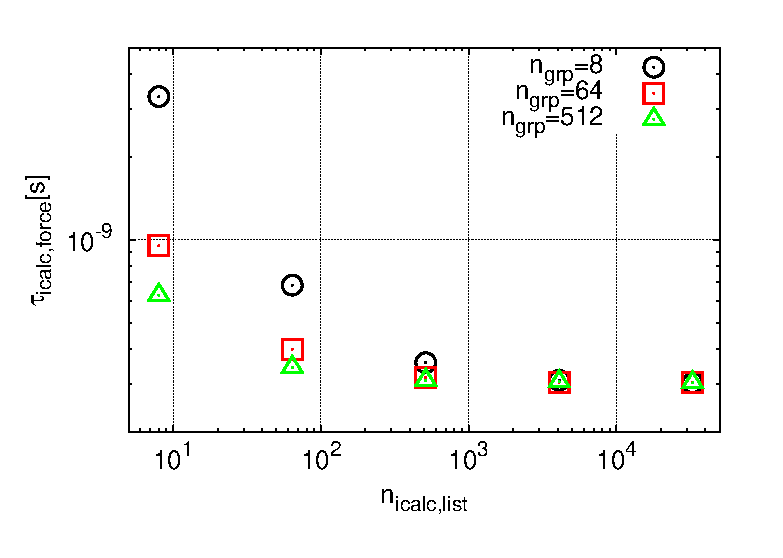
\includegraphics[width=8cm]{figure/performance/calc_force.eps}
  \end{center}
  \caption{
  
  Time for the evaluation of one gravity force against $n_{\rm icalc,
  list}$ for various $n_{\rm grp}$.
  
    }
  \label{fig:calc_force}
\end{figure}




\subsection{Total time}
\label{sec:total_time}

Now we can predict the total time of the calculation using the above
discussions. The total time per one timestep is given by
\begin{eqnarray}
  T_{\rm step} &\sim& T_{\rm dc,sort}/n_{\rm dc} \nonumber
                  + k_{\rm type}\left( T_{\rm exch,const}+T_{\rm exch,comm} \right) \nonumber \\
                  &&+ T_{\rm icalc,force} + T_{\rm icalc,const} \label{eq:totalcost2} \\
             &\sim& \tau_{\rm dc,sort} n_{\rm smp} n_p^{2/3}/n_{\rm dc} \nonumber \\
                &&+ k_{\rm type}\left( \tau_{\rm exch,const} n_{\rm exch,list} + \tau_{\rm alltoallv,startup}n_p + \tau_{\rm alltoallv,word}n_{\rm exch,list}b_pn_p^{1/3} \right) \nonumber \\
                && + \tau_{\rm icalc,force} n n_{\rm icalc,list} \nonumber \\
                && + \tau_{\rm icalc,const} n n_{\rm icalc,list} / n_{\rm grp}.   \label{eq:totalcost3}
\end{eqnarray}
The time coefficients in equation (\ref{eq:totalcost3}) for K computer
are summarized in table \ref{table:time_coefficients}. In this section
we use $n_{\rm dc}=1$.

\begin{table}
\caption{Time coefficients in equation (\ref{eq:totalcost3}) for K computer.
$\tau_{\rm icalc,force}$ is the value for gravity.  }
\begin{tabular}{|l|l|} \hline
$\tau_{\rm alltoallv,startup}$ [s] & $1.66 \times 10^{-6}$ \\ 
$\tau_{\rm alltoallv,word}$ [s/byte] & $1.11 \times 10^{-10}$\\
$\tau_{\rm dc,sort}$ [s] & $2.67\times 10^{-7}$ \\ 
$\tau_{\rm exch,const}$ [s] & $1.12 \times 10^{-7}$ \\
$\tau_{\rm icalc,const}$ [s] & $3.72\times 10^{-8}$ \\
$\tau_{\rm icalc,force}$ [s] & $3.05\times 10^{-10}$ \\ \hline
\end{tabular}
\label{table:time_coefficients}
\end{table}

To see if the predicted time by equation (\ref{eq:totalcost3}) is
reasonable, we compare the predicted time and the time obtained from
the disk galaxy simulation with the total number of particles ($N$) of
550 million and $\theta = 0.4$. In our simulations, we use up to the
quadrupole moment. On the other hand, we assume the monopole moment
only in equation (\ref{eq:totalcost3}). Thus we have to correct the
time for the force calculation in equation (\ref{eq:totalcost3}). In
our simulations, the cost of the force calculation of the quadrupole
moment is two times higher than that of the monopole moment and about
75\% of particles in the interactions list are superparticles.  Thus
the cost of the force calculation in the simulation is 75\% higher
than the prediction. We apply this correction to equation
(\ref{eq:totalcost3}). In
figure \ref{fig:performance_model_strong_breakdown_comp}, we plot the
breakdown of the predicted time with the correction and the obtained
time from the disk galaxy simulations. We can see that our predicted
times agree with the measurements very well.

\begin{figure}
  \begin{center}
    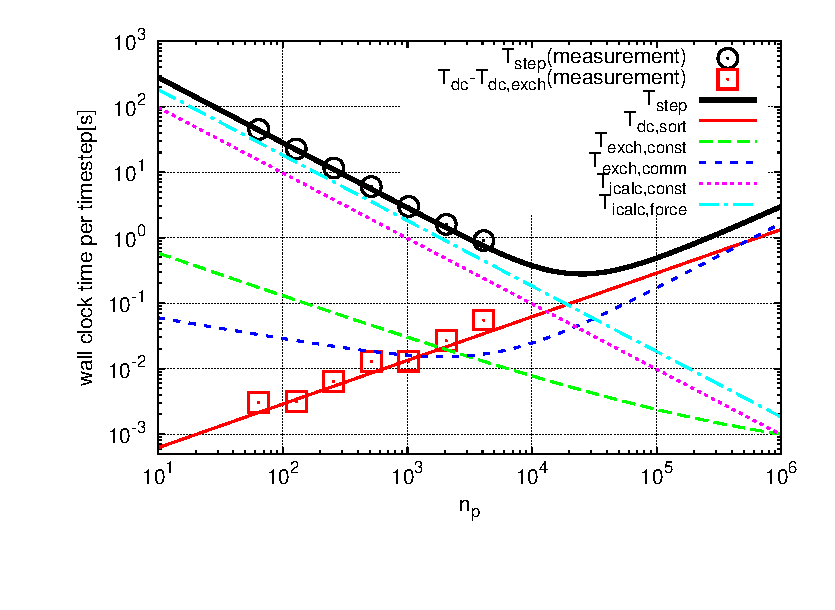
\includegraphics[width=8cm]{figure/performance/performance_model_strong_breakdown_comp.eps}
  \end{center}
  \caption{
  
  Breakdown of the total time of the calculation per one timestep
  against $n_p$, for the case of $N=5.5\times 10^8$ , $n_{\rm
  smp}=500$, $\theta=0.4$ and $n_{\rm grp}=130$.
  
}
  \label{fig:performance_model_strong_breakdown_comp}
\end{figure}

In the following, we analyze the performance of the gravitational many
body simulations for various hypothetical computers. In
figure \ref{fig:performance_model_strong_breakdown}, we plot the
breakdown of the calculation time predicted using equation
(\ref{eq:totalcost3}) for the cases of 1 billion and 10 million
particles against $n_p$. For the case of 1 billion particles, we can
see that the slope of $T_{\rm step}$ becomes shallower for
$n_p \gtrsim 10000$ and increases for $n_p \gtrsim 30000$, because
$T_{\rm dc,sort}$ dominates. Note that $T_{\rm exch,comm}$ also has
the minimum value. The reason is as follows. For small $n_p$, $T_{\rm
alltoallv,word}$ is dominant in $T_{\rm exch,comm}$ and it decrease as
$n_p$ increases, because the length of $n_{\rm exch,list}$ becomes
smaller. For large $n_p$, $T_{\rm alltoallv,startup}$ becomes dominant
and it increases linearly. We can see the same tendency for the case
of 10 million particles. However, the optimal $n_p$, at which $T_{\rm
step}$ is the minimum, is smaller than that for 1 billion particles,
because $T_{\rm dc,sort}$ is independent of $N$.


\begin{figure}
  \begin{center}
    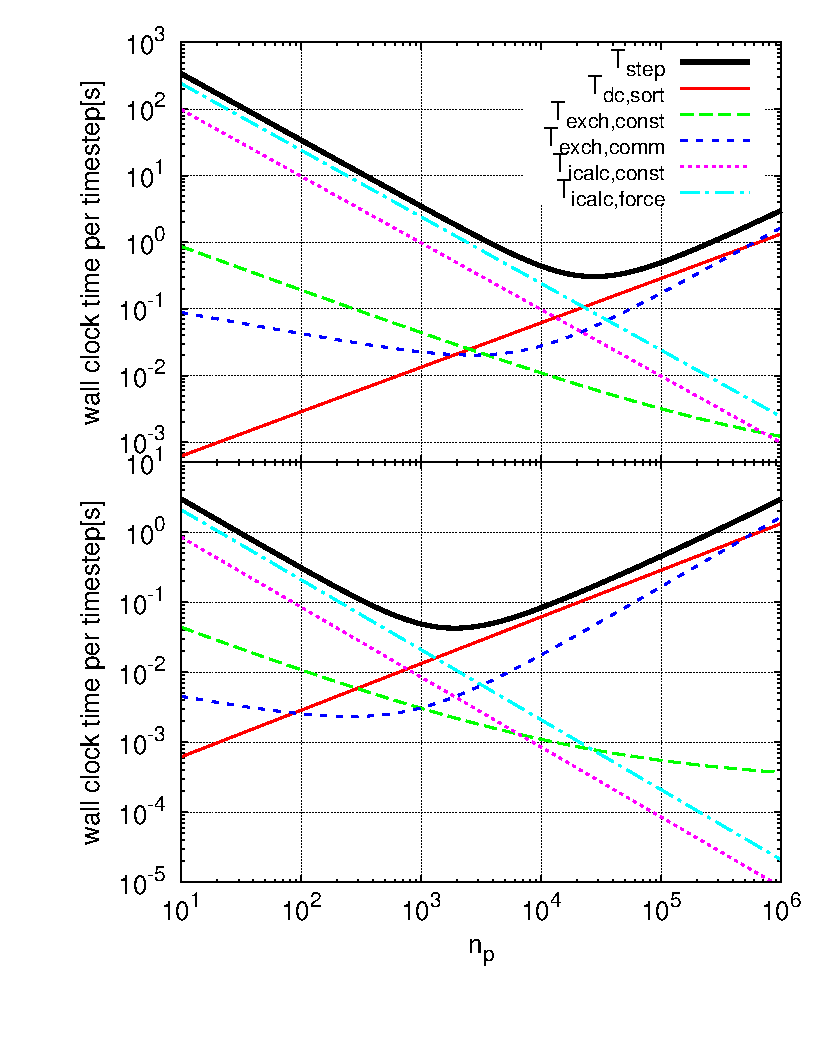
\includegraphics[width=8cm]{figure/performance/performance_model_strong_breakdown.eps}
  \end{center}
  \caption{
  
  Breakdown of the total time of the calculation per one timestep
  against $n_p$, for the case of $N=10^9$ (top panel) and $=10^7$
  (bottom panel), $n_{\rm smp}=500$, $\theta=0.4$ and $n_{\rm
  grp}=300$.
  
}
  \label{fig:performance_model_strong_breakdown}
\end{figure}

In figure \ref{fig:performance_model_strong_breakdown_x10}, we plot
the breakdown of the predicted calculation time for a hypothetical
computer which has the floating-point operation performance ten times
faster than that of K computer (hereafter X10). In other words,
$\tau_{\rm alltoallv,startup}$ and $\tau_{\rm alltoallv,word}$ are the
same as those of K computer, but $\tau_{\rm dc,sort}$, $\tau_{\rm
exch,const}$, $\tau_{\rm icalc,const}$ and $\tau_{\rm icalc,force}$
are ten times smaller than those of K computer. We can see that the
optimal $n_p$ is shifted to smaller $n_p$ for both cases of $N$ of 1
billion and 10 million, because $T_{\rm exch,comm}$ is unchanged.
However, the shortest time per timestep is improved by about a factor
of five.  If the network performance is also improved by a factor of
ten, we would get the same factor of ten improvement for the shortest
time per timestep. In other words, by reducing the network performance
by a factor of ten, we suffer only a factor of two degradation of the
shortest time.




\begin{figure}
  \begin{center} 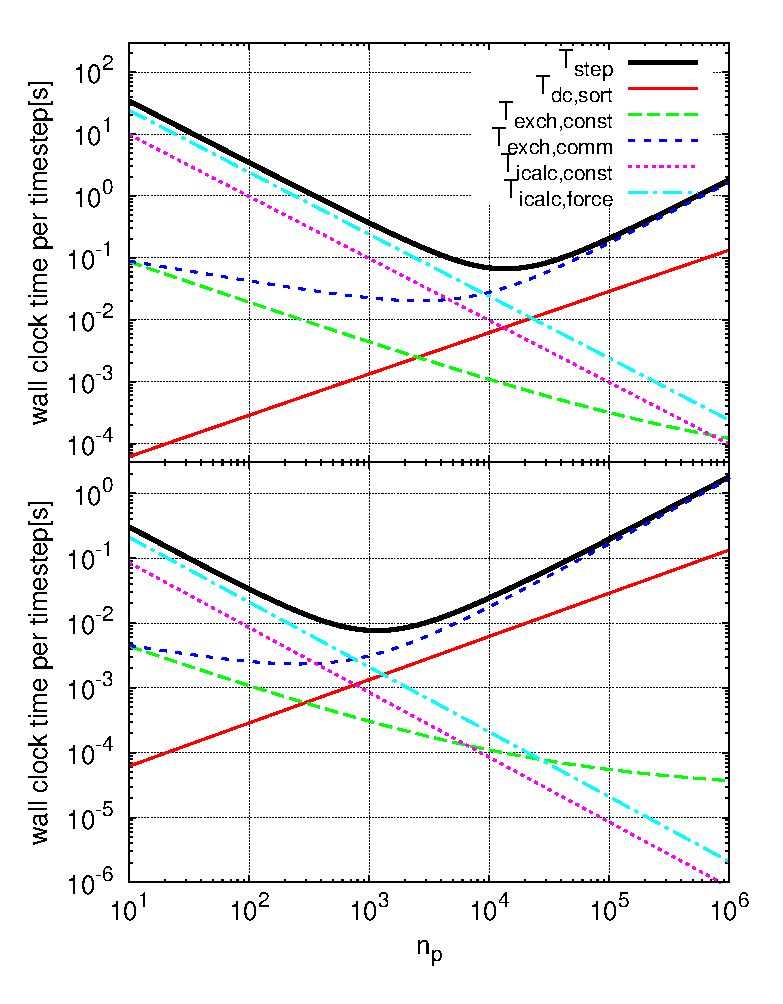
\includegraphics[width=8cm]{figure/performance/performance_model_strong_breakdown_x10.eps} \end{center} \caption{
  
The same as figure \ref{fig:performance_model_strong_breakdown}, but
for the floating-point operation performance ten times faster than K
computer.
  
}
  \label{fig:performance_model_strong_breakdown_x10}
\end{figure}

In figure \ref{fig:performance_model_strong_predict}, we plot
predicted $T_{\rm step}$ for three hypothetical computers and K
computer. Two of four computers are the same computer models we used
above. Another is a computer with the floating-point operation
performance hundred times faster than K computer (hereafter X100).
The last one is a computer of which the performance of the force
calculation is ten times faster than K computer (hereafter ACL). In
other words, only $\tau_{\rm icalc,force}$ is ten times smaller than
that of K computer.  This computer is roughly mimicking a computer
with an accelerator such as, GPU \citep{hamada2009novel},
GRAPE \citep{1990Natur.345...33S, 2003PASJ...55.1163M} and
PEZY-SC. Here we use the optimal $n_{\rm grp}$, at which $T_{\rm
step}$ is minimum, for each computers. For the case of $N=10^9$, the
optimal $n_{\rm grp} \sim 300$ for K computer and X10, $\sim 400$ for
X100 and $\sim 1600$ for ACL. For the case of $N=10^{12}$, the optimal
$n_{\rm grp}$ for K, X10, X100 is the same as those for $N=10^9$, but
$\sim 1800$ for ACL. The optimal value of $n_{\rm grp}$ for ACL is
larger than those of any other computers, because large $n_{\rm grp}$
reduces the cost of the construction of the interaction list.

From figure \ref{fig:performance_model_strong_predict}, we can see
that for small $n_p$, X10 and X100 are ten and hundred times faster
than K computer, respectively. However, for the case of $N=10^9$,
$T_{\rm step}$ of the values of X10 and X100 increase for $n_p \gtrsim
15000$ and $\gtrsim 7000$, because the $T_{\rm exch,comm}$ becomes the
bottleneck. ACL shows a similar performance to that of X10 up to
optimal $n_p$, because the force calculation is dominant in the total
calculation time. On the other hand, for large $n_p$, the performance
of ACL is almost the same as that of K computer, because ACL has the
same bottleneck as K computer has, which is the communication of the
exchange list.  On the other hand, for the case of $N=10^{12}$,
$T_{\rm step}$ is scaled up to $n_p \sim 10^5$ for all computers. This
is because for larger $N$ simulations, the costs of the force
calculation and the construction of the interaction list are
relatively higher than the communication of the exchange list. Thus
the optimal $n_p$ is sifted to larger value if we use larger $N$.



\begin{figure}
  \begin{center}
    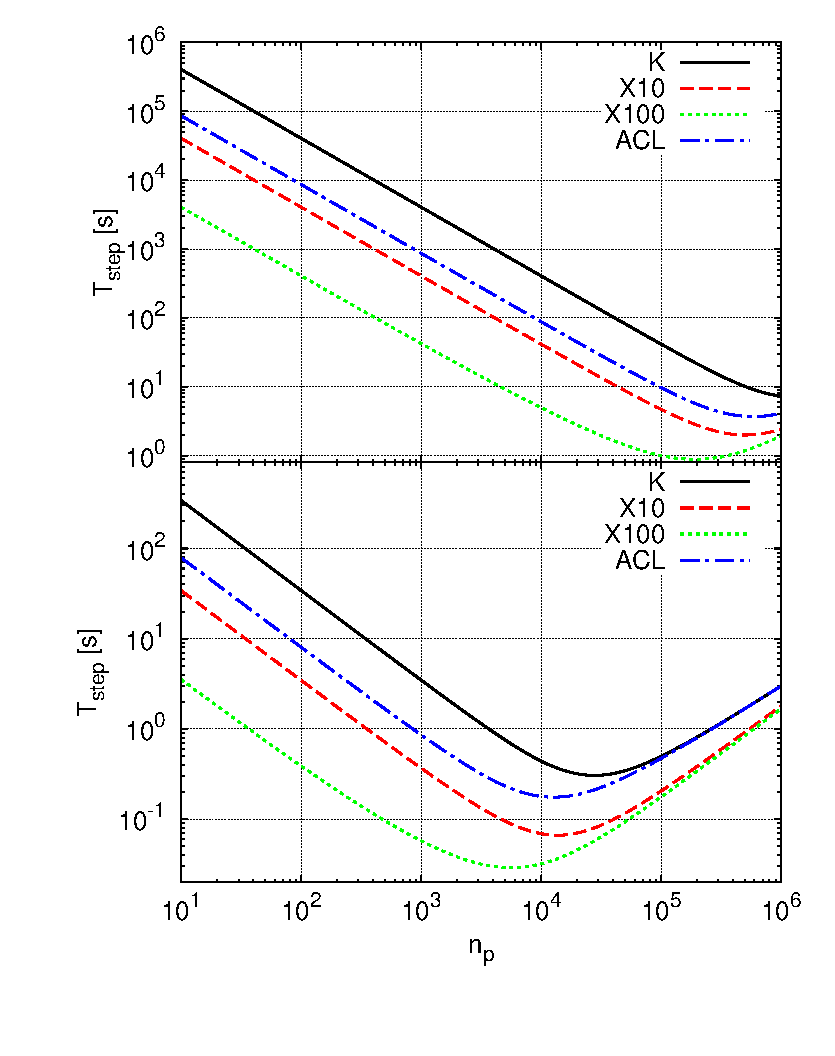
\includegraphics[width=8cm]{figure/performance/performance_model_strong_predict.eps}
  \end{center}
  \caption{
  
Predicted total calculation time for three hypothetical computers and
K computer as a function of $n_p$, for the case of $n_{\rm smp}=500$,
$\theta=0.4$.  Top and bottom panels indicate the results of the case
for $N=10^{12}$ and $N=10^{9}$, respectively.
  
}
  \label{fig:performance_model_strong_predict}
\end{figure}

From figures \ref{fig:performance_model_strong_breakdown}
and \ref{fig:performance_model_strong_breakdown_x10}, we can see that
for large $n_p$, performance will be limited by $T_{\rm dc,sort}$ and
$T_{\rm exch,comm}$. Therefor, if we can reduce them further, we can
improve the efficiency of the calculation with large $n_p$. It is
possible to reduce the time for sort by applying the algorithm used in
$x$ direction to $y$ direction as well or setting $n_{\rm dc}$ to more
than unity. It is more difficult to reduce $T_{\rm exch,comm}$, since
we are using system-provided {\tt MPI\_Alltoallv}.





\section{Conclusion}
\label{sec:conclusion}

We have developed a novel framework for particle-based simulations,
FDPS.  Users of FDPS need not care about complex implementations of
domain decomposition, exchange of particles, communication of data for
the interaction calculation, or optimization for multi-core
processors.  Using FDPS, particle simulation codes which achieve high
performance and high scalability on massively parallel
distributed-memory machines can be easily developed for a variety of
problems.  As we have shown in section~\ref{sec:samplecode}, a
parallel $N$-body simulation code can be written in less than 120
lines.  Example implementations of gravitational $N$-body simulation
and SPH simulation showed excellent scalability and performance. We
hope FDPS will help researchers to concentrate on their research, by
removing the burden of complex code development for parallization and
architecture-dependent tuning.


% LocalWords:  FDPS multi SPH parallization scalability


\bigskip

We thank M. Fujii for providing initial conditions of spiral
simulations, T. Ishiyama for providing his Particle Mesh code,
K. Yoshikawa for providing his TreePM code and Y. Maruyama for being
the first user of FDPS.  We are grateful to M. Tsubouchi for her help
in managing the FDPS development team. This research used
computational resources of the K computer provided by the RIKEN
Advanced Institute for Computational Science through the HPCI System
Research project (Project ID:ra000008). Part of the research covered
in this paper research was funded by MEXT's program for the
Development and Improvement for the Next Generation Ultra High-Speed
Computer System, under its Subsidies for Operating the Specific
Advanced Large Research Facilities. Numerical computations were in
part carried out on Cray XC30 at Center for Computational
Astrophysics, National Astronomical Observatory of Japan.


\begin{thebibliography}{}
\bibitem[Abrahama et al.(2014)]{2014GROMACS}
Abrahama,~M.~J., Murtolad,~T., Schulzb,~R., Palla,~S., Smithb,~J., Hessa,~B. \& Lindahl.,~E.\ 2015, SoftwareX, 1, 19
\bibitem[Asphaug \& Reufer(2014)]{2014NatGe...7..564A}
{{Asphaug},~E. \& {Reufer},~A.}\ 2014, Nature Geoscience, 7, 564
\bibitem[Bagla(2002)]{2002JApA...23..185B}
{Bagla},~J.~S.\ 2002, JApA, 23, 185
\bibitem[{Balsara}(1995)]{1995JCoPh.121..357B}
{Balsara},~D.~S.\ 1995, JCoPh, 121, 357
\bibitem[Barnes \& Hut(1986)]{1986Natur.324..446B}
{Barnes},~J. and {Hut},~P.\ 1986, Nature, 324, 446
\bibitem[Barnes(1990)]{1990JCoPh..87..161B}
{Barnes},~J.\ 1990, JCoPh, 87, 161
\bibitem[{B{\'e}dorf} et al.(2012)]{2012JCoPh.231.2825B}
{B{\'e}dorf},~J., {Gaburov},~E. \& {Portegies Zwart},~S.\ 2012, JCoPh, 231, 2825
\bibitem[B{\'e}dorf et al.(2014)]{Bedorf:2014:PGT:2683593.2683600}
B{\'e}dorf,~J., Gaburov,~E., Fujii,~M., Nitadori,~K., Ishiyama,~T., \& Portegies Zwart,~S.\ 2014, Proceedings of the International Conference for High Performance Computing, Networking, Storage and Analysis, IEEE Press, 54
\bibitem[Benz et al.(1986)]{1986Icar...66..515B}
{{Benz},~W., {Slattery},~W.~L. \& {Cameron},~A.~G.~W.}\ 1986, \icarus, 66, 515
\bibitem[Blackston \& Suel(1997)]{Blackston:1997:HPE:509593.509597}
Blackston,~D., \& Suel,~T.\ 1997, Proc. of the ACM/IEEE Conf. on Supercomputing, ACM, 1
\bibitem[Bode et al.(2000)]{2000ApJS..128..561B}
{Bode},~P., {Ostriker},~J.~P. \& {Xu},~G.\ 2000, ApJS, 128, 561
\bibitem[Brooks et al. (2009)]{2009CHARMM}
Brooks,~B., et al.\ 2009, J. Comp. Chem. 30, 1545
\bibitem[Cameron \& Ward(1976)]{1976LPI.....7..120C}
{{Cameron},~A.~G.~W. \& {Ward},~W.~R.}\ 1976, Lunar and Planetary Science Conference, 7, 120
\bibitem[Canup et al.(2013)]{2013Icar..222..200C}
{{Canup},~R.~M., {Barr},~A.~C. \& {Crawford},~D.~A.}\ 2013, \icarus, 222, 200
\bibitem[Case et al.(2015)]{2015AMBER}
Case,~D.~A., et al. 2015, AMBER 2015, (San Francisco:University of California)
\bibitem[Dehnen \& Aly(2012)]{2012MNRAS.425.1068D}
{{Dehnen},~W. \& {Aly},~H.}\ 2012, \mnras, 425, 1068
\bibitem[Dehnen(2000)]{2000ApJ...536L..39D}
Dehnen,~W.\ 2000, \apjl, 536, L39
\bibitem[Dubinski(1996)]{1996NewA....1..133D}
{Dubinski},~J.\ 1996, NewA, 1, 133,
\bibitem[Dubinski et al.(2004)]{2004NewA....9..111D}
Dubinski,~J., Kim,~J., Park,~C. \& Humble,~R.\ 2004, NewA, 9, 111
\bibitem[Fujii et al.(2011)]{2011ApJ...730..109F}
{Fujii},~M.~S., {Baba},~J., {Saitoh},~T.~R., {Makino},~J., {Kokubo},~E., \& {Wada},~K.\ 2011, ApJ, 730, 109
\bibitem[Gaburov et al.(2009)]{2009NewA...14..630G}
{Gaburov},~E., {Harfst},~S. \& {Portegies Zwart},~S.\ 2009, NewA, 14, 630
\bibitem[Goodale et al.(2003)]{2003Cactus}
Goodale,~T., Allen,~G., Lanfermann,~G., Mass{\'o},~J., Radke,~T., Seidel,~E. \& Shalf,~J.\ 2003, 5th International Conference, Lecture Notes in Computer Science, 2565
\bibitem[Hamada et al.(2009a)]{Hamada:2009:THN:1654059.1654123}
Hamada,~T., Narumi,~T., Yokota,~R., Yasuoka,~K., Nitadori,~K., \& Taiji,~M.\ 2009, Proceedings of the Conference on High Performance Computing Networking, Storage and Analysis, 62, 1  
\bibitem[Hamada et al.(2009b)]{hamada2009novel}
Hamada,~T., Nitadori,~K., Benkrid,~K., Ohno,~Y., Morimoto,~G., Masada,~T., Shibata,~Y., Oguri,~K. \& Taiji,~M.\ 2009, Computer Science-Research and Development, 24, 21
\bibitem[Hamada \& Nitadori(2010)]{Hamada:2010:TAN:1884643.1884644}
Hamada,~T., \& Nitadori,~K.\ 2010, Proceedings of the ACM/IEEE International Conference for High Performance Computing, Networking, Storage and Analysis, IEEE Computer Society, 1
\bibitem[{Hartmann} \& {Davis}(1975)]{1975Icar...24..504H}
{{Hartmann},~W.~K. \& {Davis},~D.~R.}\ 1975, \icarus, 24, 504
\bibitem[{Hernquist}(1990)]{1990ApJ...356..359H}
{Hernquist},~L.\ 1990, ApJ, 356, 359
\bibitem[Hockney \& Eastwood(1988)]{hockney1988computer}
Hockney,~R.~W. \& Eastwood,~J.~W.\ 1988, Computer Simulation Using Particles, CRC Press
\bibitem[Ishiyama et al.(2009)]{2009PASJ...61.1319I}
{Ishiyama},~T., {Fukushige},~T. \& {Makino},~J.\ 2009, PASJ, 61, 1319
\bibitem[Ishiyama et al.(2012)]{Ishiyama:2012:PAN:2388996.2389003}
Ishiyama,~T., Nitadori,~K., \& Makino, J.\ 2012, Proceedings of the International Conference on High Performance Computing, Networking, Storage and Analysis, 5, 1
\bibitem[Iwasawa et al.(2015)]{2015FDPS}
Iwasawa,~M., Tanikawa,~A., Hosono,~N., Nitadori,~K., Muranushi,~T. \& Makino,~J.\ 2015, WOLFHPC '15, 1, 1
\bibitem[Navarro et al.(1996)]{1996ApJ...462..563N}
{{Navarro},~J.~F., {Frenk},~C.~S. \& {White},~S.~D.~M.}\ 1996, ApJ, 462, 563
\bibitem[Nitadori et al.(2006)]{2006NewA...12..169N}
{Nitadori},~K., {Makino},~J. \& {Hut},~P.\ 2006, NewA, 12, 169
\bibitem[{Makino}(1991)]{1991PASJ...43..859M}
{Makino},~J.\ 1991, PASJ, 43, 859
\bibitem[Makino et al.(2003)]{2003PASJ...55.1163M}
Makino,~J., Fukushige,~T., Koga,~M., \& Namura,~K.\ 2003, \pasj, 55, 1163
\bibitem[Makino(2004)]{2004PASJ...56..521M}
{Makino},~J.\ 2004, \pasj, 56, 521  
\bibitem[Monaghan(1992)]{1992ARA&A..30..543M}
{Monaghan},~J.~J.\ 1992, ARA\&A, 30, 543
\bibitem[{Monaghan}(1997)]{1997JCoPh.136..298M}
{Monaghan},~J.~J.\ 1997, J. Comp. Phys., 136, 298
\bibitem[Murotani et al.(2014)]{2014Murotani}
Murotani,~K., et al.\ 2014, Journal of Advanced Simulation in Science and Engineering, 1, 16
\bibitem[Phillips et al.(2005)]{2005NAMD}
Phillips,~J., et al.\ 2005 J. Comp. Chem., 26, 1781
\bibitem[Plimpton(1995)]{1995LAMMPS}
Plimpton,~S.\ 1995, J. Comp. Phys., 117, 1
\bibitem[{Rosswog}(2009)]{2009NewAR..53...78R}
{Rosswog},~S.\ 2009, NewAR, 53, 78
\bibitem[Salmon \& Warren(1994)]{1994JCoPh.111..136S}
{Salmon},~J.~K. \& {Warren},~M.~S.\ 1994, 111, 136,
\bibitem[Schuessler \& Schmitt(1981)]{1981A&A....97..373S}
{Schuessler},~I. \& {Schmitt}, D.\ 1981, A\&A, 97, 3735
\bibitem[Shaw et al.(2014)]{GB14}
Shaw,~D.~E., et al.\ 2014, Proceedings of the International Conference on High Performance Computing, Networking, Storage and Analysis, 41
\bibitem[Springel(2005)]{2005MNRAS.364.1105S}
{Springel},~V.\ 2005, \mnras, 364, 1105
\bibitem[Springel et al.(2005)]{2005Natur.435..629S}
{Springel},~V., et al., 2005, \nat, 435, 629
\bibitem[{Springel}(2010)]{2010ARA&A..48..391S}
{Springel},~V.\ 2010, ARA\&A, 48, 391
\bibitem[Sugimoto et al.(1990)]{1990Natur.345...33S}
Sugimoto,~D., et al.\ 1990, \nat, 345, 33
\bibitem[Tanikawa et al.(2012)]{2012NewA...17...82T}
{Tanikawa},~A., {Yoshikawa},~K., {Okamoto},~T. \& {Nitadori},~K.\ 2012, NewA, 17, 82
\bibitem[Tanikawa et al.(2013)]{2013NewA...19...74T}
{Tanikawa},~A., {Yoshikawa},~K., {Nitadori},~K. \& {Okamoto},~T.\ 2013, NewA, 19, 74
\bibitem[Teodoro et al.(2014)]{2014LPI....45.2703T}
{{Teodoro},~L.~F.~A., {Warren},~M.~S., {Fryer},~C., {Eke},~V. \& {Zahnle},,K.}\ 2014, Lunar and Planetary Science Conference, 45, 2703
\bibitem[{Wadsley} et al.(2004)]{2004NewA....9..137W}
{Wadsley},~J.~W., {Stadel},~J. \& {Quinn},~T.\ 2004, NewA, 9, 137
\bibitem[Warren \& Salmon(1995)]{1995CoPhC..87..266W}
{Warren},~M.~S., \& {Salmon},~J.~K.\ 1995, Computer Physics Communications, 87, 266
\bibitem{confscWarrenSBGSW97}
M.~S.~Warren, J.~K.~Salmon, D.~J.~Becker, M.~P.~Goda, T.~L.~Sterling, \& W.~Winckelmans,\ 1997, Proceedings of the International Conference on High Performance Computing, Networking, Storage and Analysis, 61
\bibitem[Widrow \& Dubinski(2005)]{2005ApJ...631..838W}
{{Widrow},~L.~M. \& {Dubinski},~J.}\ 2005, ApJ, 631, 838
\bibitem[Xu(1995)]{1995ApJS...98..355X}
{Xu},~G.\ 1995, ApJS, 98, 355
\bibitem[Yamada et al.(2015)]{2015LexADV_EMPS}
Yamada,~T., Mitsume,~N., Yoshimura,~S. \& Murotani,~K.\ 2015, COUPLED PROBLEMS 2015
\bibitem[Yoshikawa \& Fukushige(2005)]{2005PASJ...57..849Y}
{Yoshikawa},~K. \& {Fukushige},~T.\ 2005, \pasj, 57, 849
  
\end{thebibliography}

\end{document}


